\documentclass[letterpaper,11pt]{scrreprt}
\usepackage[american]{babel}
\usepackage[latin1]{inputenc}
\usepackage[T1]{fontenc}
\usepackage[top=1in,bottom=1in,left=1in,right=1in]{geometry}
\usepackage{lmodern}

\usepackage{amsmath}
\usepackage{amssymb}

\usepackage[hyperref]{ntheorem}
\usepackage[
	bookmarks,
	colorlinks=false,
	linkcolor=blue,
	citecolor=blue,
	pagebackref=false,
	pdftitle={MADlib Design Document},
	pdfauthor={Predictive Analytics Team, Pivotal Inc.},
	pdfsubject={},
	pdfkeywords={}
]{hyperref}
\usepackage{csquotes}                  % Strongly recommended for biblatex
\usepackage[
	backend=bibtex,
	maxnames=2,
	maxbibnames=20,
	firstinits=true
]{biblatex}
\usepackage{scrpage2}                  % Headers and footers
\usepackage{color}                     % Colors, possibly only for \todo
\usepackage{enumitem}                  % enumerate environment
\usepackage{ctable}
\usepackage{tabularx}
\usepackage{xspace}                    % Correct spaces after \newcommand definitions
\usepackage[noend]{algpseudocode}      % algorithm environment
\usepackage{listings}                  % Code snippets
\usepackage{bbding}
\usepackage{latex/tikz-uml}            % UML diagrams

% BEGIN Doc Layout
	\allowdisplaybreaks[3]

	\pagestyle{scrheadings}
	\automark[chapter]{section}

	\setkomafont{disposition}{\normalcolor\bfseries}
	\setkomafont{descriptionlabel}{\bfseries}
	\setkomafont{captionlabel}{\usekomafont{disposition}}

	\setlength{\arrayrulewidth}{.5pt}
	\numberwithin{equation}{section}
	\renewcommand{\theenumi}{\roman{enumi}}
	\renewcommand{\labelenumi}{\theenumi)}

	\newcommand{\otoprule}{\midrule[\heavyrulewidth]}

	\setcounter{secnumdepth}{3}

	\makeatletter
	% Algorithms are expected to have an optional argument of form
	% FunctionName$(ArgumentList)$, e.g., DiscreteSample$(A, w)$
	\def\internal@funcName#1$(#2)${#1}
	\newcommand\funcName[1]{\internal@funcName #1}
	\newtheoremstyle{algorithm}
		{\item[\rlap{\vbox{\hbox{\hskip\labelsep \theorem@headerfont
			##1\ ##2\theorem@separator}\hbox{\strut}}}]}%
		{\item[\rlap{\vbox{\hbox{\hskip\labelsep {\theorem@headerfont
			##1}\ \normalfont\texttt{##3}{\theorem@headerfont\theorem@separator}}\hbox{\strut}}}]%
			\def\@currentlabel{\texttt{\funcName{##3}}}}
	\makeatother

	\makeatletter
	% Also display JSTOR in small caps
	% http://sourceforge.net/tracker/index.php?func=detail&aid=3152938&group_id=244752&atid=1126006
	\DeclareFieldFormat{eprint:arxiv}{%
	  \textsc{arXiv}\addcolon
	  \ifhyperref
	    {\href{http://arxiv.org/\abx@arxivpath/#1}{%
	       \nolinkurl{#1}%
	       \iffieldundef{eprintclass}
		 {}
		 {\addspace\texttt{\mkbibbrackets{\thefield{eprintclass}}}}}}
	    {\nolinkurl{#1}
	     \iffieldundef{eprintclass}
	       {}
	       {\addspace\texttt{\mkbibbrackets{\thefield{eprintclass}}}}}}
	\DeclareFieldFormat{eprint:jstor}{%
	  \mkbibacro{JSTOR}\addcolon\space
	  \ifhyperref
	    {\href{http://www.jstor.org/stable/#1}{\nolinkurl{#1}}}
	    {\nolinkurl{#1}}}
	% Some conferences do not have DOIs for their papers, but they do get
	% IDs in the ACM Digital Library. E.g., SODA papers.
	\DeclareFieldFormat{eprint:acm}{%
	  \mkbibacro{ACM}\addcolon\space
	  \ifhyperref
	    {\href{http://dl.acm.org/citation.cfm?id=#1}{\nolinkurl{#1}}}
	    {\nolinkurl{#1}}}
	\makeatother

	\newlist{moduleinfo}{description}{2}
	\setlist[moduleinfo]{style=multiline,labelindent=\leftmargini,leftmargin=3cm,rightmargin=\leftmargini,font=\bfseries}
	\newlist{modulehistory}{description}{2}
	\setlist[modulehistory]{style=multiline,leftmargin=1.1cm}
% END Doc Layout

% BEGIN General Definitions
	\newcommand{\todo}[1]{\textbf{\color{red}#1}}

	\newcommand{\specialcell}[3][t]{%
		\begin{tabular}[#1]{@{}#2@{}}#3\end{tabular}}

	% BEGIN Mathematical Definition
		% Space (only) in displaymath (e.g., between mathematical expression and punctuation mark)
		\newcommand{\SiM}{\mathchoice{\,}{}{}{}}
	% END Mathematical Operators

	% BEGIN URLs
		\newcommand{\mailto}[1]{\href{mailto:#1}{\nolinkurl{#1}}}
		\newcommand{\doi}[1]{DOI: \href{http://dx.doi.org/#1}{\nolinkurl{#1}}}
	% END URLs

	\makeatletter
	% BEGIN Mathematical Definitions
		% BEGIN Set Symbols
			\newcommand{\setsymbol}[1]{\mathbb{#1}}
			\newcommand{\N}{\@ifstar{\setsymbol{N}_0}{\setsymbol{N}}}
			\newcommand{\R}{\setsymbol{R}}
		    \newcommand{\Nupto}{\@ifstar{\Nupto@star}{\Nupto@nostar}}
		    \newcommand{\Nupto@star}[1]{[#1]_0}
		    \newcommand{\Nupto@nostar}[1]{[#1]}
		% END Set Symbols
		\renewcommand{\vec}[1]{\ensuremath{\boldsymbol{#1}}}
	% END Mathematical Definitions
	\makeatother

	\renewcommand{\vec}[1]{\ensuremath{\boldsymbol{#1}}}
	\newcommand{\enumref}[1]{(\ref{#1})}

	\makeatletter
	\newcommand{\symlabel}[2]{\def\@currentlabel{\texttt{#1}}\texttt{#1}\label{#2}}
	\makeatother

	\newcommand{\Warning}[1]{\marginpar[\HandRight]{\HandLeft}\textbf{#1}}

	% BEGIN Algorithms
	\theoremstyle{algorithm}
	\theorembodyfont{\upshape}
	\newtheorem{algorithm}{Algorithm}[section]

	\newlength{\alglabelwidth}
	\newcommand{\alginput}[1]{%
		\par\noindent%
		\settowidth{\alglabelwidth}{\emph{Output:}}%
		\makebox[\alglabelwidth][l]{\emph{Input:}} \begin{tabular}[t]{l} #1 \end{tabular}}
	\newcommand{\algoutput}[1]{%
		\par\noindent%
		\settowidth{\alglabelwidth}{\emph{Output:}}%
		\makebox[\alglabelwidth][l]{\emph{Output:}} \begin{tabular}[t]{l} #1 \end{tabular}}
	\newcommand{\algprecond}[1]{%
		\par\noindent\textit{Initialization/Precondition: #1}}

	\newcommand{\set}{\leftarrow}
	\DeclareMathOperator{\random}{random}
	\newcommand{\dist}{\ensuremath{\mathit{dist}}}
	\newcommand{\List}{\mathrm{List}}
	\newcommand{\Sample}{\mathit{Sample}}
	\algblockdefx[With]{With}{EndWith}%
		[1]{\textbf{with} #1 \textbf{do}}%
		[0]{End}
	\algnotext[With]{EndWith}
	% END Algorithms

	% BEGIN lstlisting environments
	\lstset{
		basicstyle=\ttfamily\footnotesize,       % the size of the fonts that are used for the code
		numbers=left,                   % where to put the line-numbers
		numberblanklines=false
		numbersep=1em,                  % how far the line-numbers are from the code
		basewidth=0.52em,
		tabsize=4,  		% sets default tabsize to 2 spaces
		xleftmargin=\leftmargini
	}
	\renewcommand*\thelstnumber{\the\value{lstnumber}:}
	% END lstlisting environments

	\lstnewenvironment{sql}[1][]{\lstset{language=SQL,gobble=4,emphstyle=\textit,#1}}{}
	\lstnewenvironment{cpp}[1][]{\lstset{language=C++,gobble=4,emphstyle=\textit,#1}}{}
	\lstnewenvironment{cppsnippet}[1][]{\lstset{basicstyle=\ttfamily,language=C++,stepnumber=0,gobble=8,emphstyle=\textit,xleftmargin=0pt,#1}}{}
% END General Definitions

\bibliography{../literature.bib}

% BEGIN Preamble
\title{%
	MADlib Design Document%
}

\newcommand{\bR}{\mathcal{R}}
\newcommand{\norm}[1]{\| #1 \|_2}


\begin{document}

\maketitle

\tableofcontents

% When using TeXShop on the Mac, let it know the root document. The following must be one of the first 20 lines.
% !TEX root = ../design.tex

\chapter{Abstraction Layers}

\begin{moduleinfo}
\item[Author] \href{mailto:Florian.Schoppmann@emc.com}{Florian Schoppmann}
\item[History]
	\begin{modulehistory}
		\item[v0.5] Initial revision of design document
		\item[v0.4] Support for function pointers and sparse-vectors
		\item[v0.3] C++ abstraction layer rewritten as a template library, switched to Eigen \cite{eigen} as linear-algebra library
		\item[v0.2] Initial revision of C++ abstraction layer, incorporated Armadillo \cite{armadillo} as linear-algebra library
	\end{modulehistory}
\end{moduleinfo}

% Abstract. What is the problem we want to solve?

\section{The C++ Abstraction Layer}

There are a number of complexities involved in writing C or C++-based user-defined functions over a legacy DBMS like PostgreSQL, all of which can get in the way of maintainable, portable application logic. This complexity can be especially frustrating for routines whose pseudocode amounts to a short linear-algebra expression that \emph{should} result in a compact implementation.

MADlib provides a C++ abstraction layer both to ease the burden of writing high-performance UDFs, and to encapsulate DBMS-specific logic inside the abstraction layer, rather than spreading the cost of maintenance and porting across all the UDFs in the library. In brief, the MADlib C++ abstraction currently provides five classes of functionality: type bridging, math-library integration, resource-management shims, high-level types, and templates for modular fold/reduce components.

\subsection{Overview of Functionality} \label{sec:C++AL:Classes}

\paragraph{Type Bridging}

The basic responsibility for the C++ abstraction layer is to bridge database types to native C++ types. For a DBMS, a user-defined function implemented in a compiled language is typically nothing more but a symbol (i.e., an address) in a shared library. As such, DBMS APIs specify that UDFs must have a fixed signature, and arguments are passed as an array of pointers along with additional meta data. Hand-written C code would therefore often consist of long boilerplate code that is very specific to the underlying DBMS: Making sure that the passed data is of the correct type, copying immutable data before doing modifications, verifying array lengths, etc. The C++ abstraction layer encapsulates all this within the recursive \texttt{AnyType} class that can contain either a primitive type (like, e.g., \texttt{int} or \texttt{double}) or multiple other values of type \texttt{AnyType} (for representing a composite type). This encapsulation works both for passing data from the DBMS to the C++ function, as well as returning values back from C++. To give an example: A simple, portable, and completely type-safe (though arguably not very useful) function that adds two numbers could be implemented with essentially as little code as in a high-level scripting language:
\begin{cpp}
    AnyType
    sum_two_doubles::run(AnyType& args) {
        return args[0].getAs<double>()
             + args[1].getAs<double>();
    }
\end{cpp}

\paragraph{Math-Library Integration and Performance}

SQL comes without any native support for vector and matrix operations. This presents challenges at two scales. At a macroscopic level, matrices must be intelligently partitioned into chunks that can fit in memory on a single node. At a microscopic scale, the database engine must invoke efficient linear-algebra routines on the pieces of data it gets in core. To this end, the C++ abstraction layer incorporates the very performant linear-algebra library Eigen~\cite{eigen}. Most importantly, it provides additional type bridges that do not involve memory copying and thus are very efficient: For instance, double-precision arrays in the DBMS are the canonic way to represent real-valued vectors. Therefore, the C++ abstraction layer not just provides an array-to-array bridge but also maps DBMS arrays to Eigen vectors. The bridged types can be used with all of the very sophisticated vector and matrix operations provided by Eigen.

Incorporating proven third-party libraries moreover makes it easy for MADlib developers to write correct and performant code: For instance, the Eigen linear-algebra library contains well-tested and well-tuned code that makes use of the SIMD instruction sets (like SSE) found in today's CPUs. Recent versions of Eigen even allow coupling with proprietary high-performance mathematical routines like the Intel Math Kernel Library.

Likewise, the C++ abstraction layer itself has been tuned for efficient value marshaling. Some examples include: All type bridges are aware of mutable and immutable objects and avoid making copies whenever possible. DBMS-catalogue lookups occur only once per query and are then minimized by caching. Moreover, the C++ abstraction layer is written as a template library and with the goal of reducing the runtime and abstraction overhead to a minimum. In particular, it takes extra steps to avoid memory allocation whenever possible.

\paragraph{Resource-Management Shims}

Another aspect of the C++ abstraction layer is to provide a safe and robust runtime environment with a standard interface. For instance, PostgreSQL maintains a hierarchy of memory contexts: When a query is started, a new memory context is created and all transient memory allocations are supposed to occur within this context. When the query ends, disposing of the query context provides a simple and effective way of garbage collection. The C++ abstraction layer makes sure that such modi operandi are followed. On the other hand, the C++ abstraction layer also facilitates writing C++ code with a well-defined interface. This is particularly necessary if (as is typically the case) a DBMS only provides a C plugin interface: In that case it is important that exceptions, signals, etc.\ do not cross runtime boundaries.

\paragraph{High-level types}

A second responsibility of the abstraction layer is to help compensating for SQL's lack of higher-order logic: For instance, an \texttt{AnyType} object can contain a \texttt{FunctionHandle}, which points to a user-defined function. With the syntactic sugar possible in C++, this essentially makes in-database functions first-class objects like they commonly are in modern programming languages. Internally, the abstraction layer maps UDFs to their object ID in the database, and it takes care of looking up the function in the database catalog, verifying argument lists, ensuring type-safety, etc.

Likewise, there is the need to pass internal data structures from one UDF to another (i.e., possibly through the DBMS) in a performant and portable way. While DBMSs like PostgreSQL support user-defined composite types, converting into them (or even using them in internal C++ code) is slow, creates dependencies on MADlib-specific type-bridging classes, and hinders code reuse in/from other projects than MADlib. The C++ abstraction layer therefore contains the recursive \ref{sym:DynamicStruct} class that provides a C++ struct/class interface around a stream of bytes. This class is very generic and can easily be used with any contiguous blocks of memory. Compared to the alternative of using existing serialization and deserialization classes, we expect \ref{sym:DynamicStruct} to be far better performing, as it modifies constant-length elements directly in the byte stream.

\paragraph{Modular Fold/Reduce Components}

The most basic building block in the macro-programming of MADlib is the use of user-defined aggregates (UDAs). In general, aggregates---and the related window functions---are the natural way in SQL to implement mathematical functions that take as input the values of an arbitrary number of rows. Unfortunately, concrete extension interfaces for user-defined aggregates vary widely across vendors and open-source systems. Nonetheless, the aggregation paradigm (or in functional programming terms, ``fold and reduce'') is natural and ubiquitous, and in most widely-used DBMSs (e.g., in PostgreSQL, MySQL, Greenplum, Oracle, SQL Server, Teradata) a user-defined aggregate consists of a well-known pattern of two or three user-defined functions:
\begin{enumerate}
	\item A \emph{transition function} that takes the current transition state and a new data point. It combines both into into a new transition state. The transition function is equivalent to the ``combining'' function passed to linear \emph{left-fold} functions in functional-programming languages.
	\item An optional \emph{merge function} that takes two transition states and computes a new combined transition state. This function is only needed for parallel execution. In functional-programming terms, a merge operation is a tree-like fold.
	\item A \emph{final function} that takes a transition state and transforms it into the output value.
\end{enumerate}
Clearly, a user-defined aggregate is inherently data-parallel if the transition function is associative and the merge function returns the same result as if the transition function was called repeatedly for every individual element in the second state.

Since the fold/reduce computational model is so ubiquitous and we anticipate the need to share code with other projects, fold/reduce code should not be interwoven with the DBMS interface. That is, fold/reduce-components should be implemented as independent C++ classes (possibly as generic template classes), without dependencies on MADlib-specific type-bridging classes like \texttt{AnyType}. However, fold/reduce components need to store their state as objects that the backend can understand---for maximum portability, all state information must even reside in a single contiguous block of memory. The C++ abstraction layer therefore provides a recursive class \texttt{DynamicStruct} that can contain objects both of primitive data types as well as objects of variable length, including other objects of \texttt{DynamicStruct}. This solution is more performant than serialization and deserialization, because it allows fixed-length datums to be modified directly in the block of memory.


\subsection{Type Bridging}

\subsubsection[Class AnyType]{Class \symlabel{AnyType}{sym:AnyType}}

\ref{sym:AnyType} is a container type for all values that are passed between the DBMS and C++ code. This also includes values passed to or returned from UDFs invoked as \ref{sym:FunctionHandle}. An \ref{sym:AnyType} object represents one of three kinds of values:
%
\begin{enumerate}
	\item NULL
	\item A simple value. E.g., this may be a value of a primitive data type like \texttt{int} or \texttt{double}, or a value of some abstraction-layer type like \ref{sym:FunctionHandle}.
	\item A composite value (i.e., a tuple). In this case, the \ref{sym:AnyType} object contains a list of other \ref{sym:AnyType} objects. Tuple elements are not named but instead accessed by index.
\end{enumerate}
%
\ref{sym:AnyType} objects should be explicitly instantiated only for returning values to the backend or for invoking a \ref{sym:FunctionHandle}. Implementations may choose to have different internal representations for values received from the backend and values from UDF code. The two constructors below only pertain to instantiations within UDF code. Constructors used by internal abstraction-layer code are implementation-specific.

\paragraph{Member functions}

\begin{itemize}
	\item
		\begin{cppsnippet}
		AnyType()
		\end{cppsnippet}

		Default constructor. Initializes this object as NULL. This constructor must also be used for initializing a composite object. After construction, \texttt{operator<\/<()} can be used to append values to the composite object.

	\item
		\begin{cppsnippet}
		template <class T> AnyType(const T& inValue)
		\end{cppsnippet}
		
		Template constructor (will not be used as copy constructor). This constructor will be invoked when initializing this object with an arbitrary value (excluding composite types).

	\item
		\begin{cppsnippet}
		template <class T> T getAs()
		\end{cppsnippet}
		
		Convert this object to the type specified as template argument.

	\item
		\begin{cppsnippet}
		AnyType operator[](uint16_t inID) const
		\end{cppsnippet}
		
		If this object is a composite value, return the element with index \texttt{inID}. To the user, \ref{sym:AnyType} is a fully recursive type: An \ref{sym:AnyType} object may contain a composite value, in which case it is composed of a number of other AnyType objects.
		
		This method will raise an error if this object does not contain a composite value.

	\item
		\begin{cppsnippet}
		uint16_t numFields() const
		\end{cppsnippet}

		Return the number of elements in the tuple. If this object contains NULL, return 0; if it contains a simple value, return 1.

	\item
		\begin{cppsnippet}
		bool isNull() const
		\end{cppsnippet}
		
		Return if this object is NULL.

	\item
		\begin{cppsnippet}
		bool isComposite() const
		\end{cppsnippet}
		
		Return if this object is a composite value.

	\item
		\begin{cppsnippet}
		AnyType& operator<<(const AnyType& inValue)
		\end{cppsnippet}
		
		If this object is NULL, or a composite value that has previously been constructed with the default constructor, add an element to this object. Otherwise, raise an error.
\end{itemize}

\paragraph{Non-Member Functions}

\begin{itemize}
	\item
		\begin{cppsnippet}
		AnyType Null()
		\end{cppsnippet}

		Return an AnyType object representing NULL.
	
	\item
		\begin{cppsnippet}
		template <class T> T AnyType_cast(const AnyType& inValue)
		template <class T> T AnyType_cast(const T& inValue)
		template <class T> T AnyType_cast(T& inValue)
		\end{cppsnippet}
		
		Explicit cast that converts \ref{sym:AnyType} objects to a target type \texttt{T}, but leaves values that already are of type \texttt{T} unaffected.
		
		Sometimes it is desirable to write generic code that works on both an \ref{sym:AnyType} object as well as a value with a concrete type. For instance, a \ref{sym:FunctionHandle} always returns an \ref{sym:AnyType} object. In generic code, however, a \ref{sym:FunctionHandle} might as well be replaced by just a call to a ``normal'' functor or a C++ function pointer, both of which typically return concrete types (e.g., \texttt{double}).
		
		In generic code, we could write \texttt{AnyType\_cast<double>(func())} so that if the template type of \texttt{func} is a \ref{sym:FunctionHandle}, we have an explicit conversion to \texttt{double}, whereas if \texttt{func} is just a function pointer, the return value of \texttt{func()} passes unchanged.
\end{itemize}


\subsection{Math-Library Integration}

\subsubsection[Class HandleMap]{Class \symlabel{HandleMap}{sym:HandleMap}}

\paragraph{Requirements}

\begin{itemize}
	\item \texttt{EigenType} The Eigen type that this \ref{sym:HandleMap} will wrap. Examples are \texttt{Eigen::VectorXd} or \texttt{Eigen::MatrixXd}.
	\item \texttt{Handle} Type conforming to \ref{sym:ContiguousDataHandle} concept. The two types \texttt{EigenType::Scalar} and \texttt{Handle::element\_type} must coincide.
	\item \texttt{MapOptions} Passed as template parameter \texttt{MapOptions} to \texttt{Eigen::Map}.
\end{itemize}

\paragraph{Types}

\begin{itemize}
	\item \texttt{Index}: \texttt{EigenType::Index}
\end{itemize}

\paragraph{Member functions}

\begin{itemize}
	\item
		\begin{cppsnippet}
		// constructors
		HandleMap(const Handle& inHandle) // (1)
		HandleMap(const Eigen::MapBase<Derived>& inMappedData) // (2)
		HandleMap(const Handle &inHandle, Index inNumElem) // (3)
		HandleMap(const Handle &inHandle, Index inNumRows, Index inNumCols) // (4)
		\end{cppsnippet}
	
		Constructor (1) constructs an empty \ref{sym:HandleMap} that points to NULL. Constructor (2) constructs a \ref{sym:HandleMap} that is backed by a contiguous memory block within an existing Eigen matrix (or vector). Note that not all of Eigen's block operations return contiguous memory blocks. E.g., while the \texttt{col()} method returns contiguous blocks if column-oriented storage is used, the \texttt{row()} method does not! Constructor (3) and (4) construct a \ref{sym:HandleMap} that is backed by a \texttt{Handle}.
	
	\item
		\begin{cppsnippet}
		HandleMap& operator=(const HandleMap& other)
		\end{cppsnippet}
		
		Assign another \ref{sym:HandleMap} to this object. This does not change any references or pointers, but copies all elements, i.e., the behavior is identical to other Eigen objects.
	
	\item
		\begin{cppsnippet}
		HandleMap& rebind(const Handle& inHandle);
		HandleMap& rebind(const Handle& inHandle, Index inSize);
		HandleMap& rebind(const Handle& inHandle, Index inRows, Index inCols);
		HandleMap& rebind(Index inSize);
		HandleMap& rebind(Index inRows, Index inCols);
		\end{cppsnippet}
		
		Change the handle that is backing this object. All except the first form may also be used to change the dimensions of the matrix (or vector) represented by this object.
\end{itemize}

\paragraph{Concrete Types}

\begin{itemize}
	\item \texttt{MappedMatrix}: \texttt{HandleMap<const Matrix, TransparentHandle<double> >}
	\item \texttt{MutableMappedMatrix}: \texttt{HandleMap<Matrix, TransparentHandle<double, Mutable> >}
	\item \texttt{NativeMatrix}: \texttt{HandleMap<const Matrix, ArrayHandle<double> >}
	\item \texttt{MutableNativeMatrix}: \texttt{HandleMap<Matrix, MutableArrayHandle<double> >}
	\item The corresponding four definitions for \texttt{ColumnVector} instead of \texttt{Matrix}.
\end{itemize}


\subsection{Resource-Management Shims}

\subsubsection[Class Allocator]{Class \symlabel{Allocator}{sym:Allocator}}

\paragraph{Member functions}

\subsubsection[Class NativeRandomNumberGenerator]{Class \symlabel{NativeRandomNumberGenerator}{sym:NativeRandomNumberGenerator}}

\paragraph{Member functions}


\subsection{High-Level Types}

\subsubsection[Class FunctionHandle]{Class \symlabel{FunctionHandle}{sym:FunctionHandle}}

A \ref{sym:FunctionHandle} is a function ``pointer'' to a UDF. A compliant implementation might just store the object ID of the UDF in the database, and upon invocation look up the function in the database catalog, do argument verification, retrieve a function pointer in memory and finally invoke this function pointer.

There are several options for implementations to improve performance. First, if function \texttt{funcPtr()} returns a non-NULL value, the UDF is implemented using the C++ abstraction layer and can be called directly, without going through the usual backend functions. Second, the \texttt{invoke} function is \emph{not} \texttt{const}, so implementations can cache metadata (and therby modify the \ref{sym:FunctionHandle} object).

\paragraph{Types}

\begin{itemize}
	\item
		\texttt{udf\_ptr}: \texttt{AnyType (*)(AnyType\&)}
\end{itemize}

\paragraph{Member functions}

\begin{itemize}
	\item
		\begin{cppsnippet}
		udf_ptr funcPtr();
		\end{cppsnippet}

		If the UDF is a function written using the C++ abstraction layer, implementations may return a pointer to the C++ function. Alternatively, an implementation may always return NULL. Callers must not rely on \texttt{funcPtr} returning non-NULL values.

	\item
		\begin{cppsnippet}
		FunctionHandle& setFunctionCallOptions(uint32_t inFlags)
		FunctionHandle& unsetFunctionCallOptions(uint32_t inFlags)
		uint32_t getFunctionCallOptions() const
		\end{cppsnippet}
		
		Set or get the current function call options. Options are a bit field of properties as defined above.
	
	\item
		\begin{cppsnippet}
		AnyType invoke(AnyType& args)
		\end{cppsnippet}
		
		Invoke the UDF with the given arguments. Note that \texttt{args} has to be a composite value.
	
	\item
		\begin{cppsnippet}
		AnyType operator()()
		AnyType operator()(AnyType& arg1, ..., AnyType& argn)
		\end{cppsnippet}
		
		Convenience method. Call \texttt{invoke} with the given arguments combined into one composite value.
\end{itemize}


\subsubsection[Concept ContiguousDataHandle]{Concept \symlabel{ContiguousDataHandle}{sym:ContiguousDataHandle}}

A \ref{sym:ContiguousDataHandle} is an opaque pointer to contiguous data that may be augmented by metadata. For instance, a \ref{sym:ContiguousDataHandle} may wrap a DBMS-native array that contains both a pointer to the array data, as well as information about the array's size. Since elements are stored contiguously, they can also be accessed using offsets on regular pointers to elements.

\paragraph{Requirements}

\begin{itemize}
	\item \texttt{T} Element type
\end{itemize}

\paragraph{Types}

\begin{itemize}
	\item
		\texttt{element\_type}: \texttt{T}
\end{itemize}

\paragraph{Member Functions}

\begin{itemize}
	\item
		\begin{cppsnippet}
		const element_type* ptr() const
		\end{cppsnippet}

		Return a pointer to the first element.

	\item
		\begin{cppsnippet}
		const element_type& operator[](size_t inIndex) const
		\end{cppsnippet}

		Return an element.
\end{itemize}

\paragraph{Specialized Concepts}

The concept \symlabel{MutableContiguousDataHandle}{sym:MutableContiguousDataHandle} contains also the following non-const member functions:
%
\begin{itemize}
	\item
		\begin{cppsnippet}
		element_type* ptr()
		\end{cppsnippet}

	\item
		\begin{cppsnippet}
		element_type& operator[](size_t inIndex)
		\end{cppsnippet}
\end{itemize}
%
The concept \symlabel{SizedContiguousDataHandle}{sym:SizedContiguousDataHandle} contains also the following member function:
%
\begin{itemize}
	\item
		\begin{cppsnippet}
		size_t size() const
		\end{cppsnippet}
		
		Return the number of elements in this object.
\end{itemize}
%
The concept \symlabel{MutableSizedContiguousDataHandle}{sym:MutableSizedContiguousDataHandle} combines both \ref{sym:MutableContiguousDataHandle} and \ref{sym:SizedContiguousDataHandle}.

\subsubsection[Class Ref]{Class \symlabel{Ref}{sym:Ref}}

\ref{sym:Ref} objects are conceptually equivalent to normal C++ references. However, they allow \emph{rebinding} to a different target.

\paragraph{Requirements}

\begin{itemize}
	\item \texttt{T} Target type
	\item \texttt{IsMutable} Boolean parameter indicating if objects of this type can be used to modify the target
\end{itemize}

\paragraph{Types}

\begin{itemize}
	\item
		\texttt{value\_type}: \texttt{T}
\end{itemize}

\paragraph{Member Functions}

\begin{itemize}
	\item
		\begin{cppsnippet}
		Ref& rebind(val_type* inPtr)
		\end{cppsnippet}

		Rebind this reference to a different target.

	\item
		\begin{cppsnippet}
		operator const val_type&() const
		\end{cppsnippet}

		Return a const-reference to the target.

	\item
		\begin{cppsnippet}
		const val_type* ptr() const
		\end{cppsnippet}

		Return a const-pointer to the target.
	
	\item
		\begin{cppsnippet}
		bool isNull() const
		\end{cppsnippet}

		Return if this reference has been bound to a target.
\end{itemize}

If \texttt{IsMutable == true}, then \ref{sym:Ref} also contains the following non-const member functions:

\begin{itemize}
	\item \texttt{operator val\_type\&()}
	\item \texttt{val\_type* ptr()}
\end{itemize}

Moreover it contains:
\begin{itemize}
	\item
		\begin{cppsnippet}
		Ref& operator=(Ref& inRef)
		Ref& operator=(const val_type& inValue)
		\end{cppsnippet}
		
		Assign the target value of \texttt{inRef} or \texttt{inValue} to the target of this object.
		
		It is important to define the first assignment operator because C++ will otherwise perform an assignment as a bit-by-bit copy. Note that this default \texttt{operator=} would be used even though there is a conversion path through \texttt{dest.operator=(orig.operator const val\_type\&())}.
\end{itemize}


\subsubsection[Class ByteStream]{Class \symlabel{ByteStream}{sym:ByteStream}}

\ref{sym:ByteStream} objects are similar to \texttt{std::istream} objects in that they are used to \emph{bind} (as opposed to \emph{read} in the case of \texttt{std::istream}) references to positions in byte sequences. \texttt{operator>\/>()} functions are provided for users of \ref{sym:ByteStream} objects. Each \ref{sym:ByteStream} object controls a \ref{sym:ByteStreamHandleBuf}, which in turn controls a block of memory (the storage/buffer) and has a current position.

A \ref{sym:ByteStream} object can be in \emph{dry-run} mode, in which case \texttt{operator>\/>} invocations move the current position, but no rebinding takes place. Dry-run mode is used, e.g., to determine the storage size needed to hold a \ref{sym:DynamicStruct}.

\paragraph{Member Functions}

\begin{itemize}
	\item
		\begin{cppsnippet}
		template <size_t Alignment>
		size_t seek(std::ptrdiff_t inOffset, std::ios_base::seekdir inDir) // (1)
		size_t seek(size_t inPos) // (2)
		size_t seek(std::ptrdiff_t inOffset, std::ios_base::seekdir inDir) // (3)
		\end{cppsnippet}
		
		Move the current position in the stream. Variant (1) rounds the new position up to the next multiple of \texttt{Alignment}.
	
	\item
		\begin{cppsnippet}
		size_t available() const
		\end{cppsnippet}
		
		Return the number of characters between the current position and the end of the stream.
		
	\item
		\begin{cppsnippet}
		const char_type* ptr() const
		\end{cppsnippet}
		
		Return a pointer to the beginning of the buffer.
	
	\item
		\begin{cppsnippet}
		size_t size() const
		\end{cppsnippet}
		
		Return the size of the buffer.
	
	\item
		\begin{cppsnippet}
		size_t tell() const
		\end{cppsnippet}
	
	\item
		\begin{cppsnippet}
		std::ios_base::iostate rdstate() const
		bool eof() const
		\end{cppsnippet}
	
		Return status information about the stream, in a fashion similar to \texttt{std::istream}.
	\item
		\begin{cppsnippet}
		bool isInDryRun() const
		\end{cppsnippet}
	
		Return if the stream is in dry-run mode.

	\item
		\begin{cppsnippet}
		template <class T> const T* read(size_t inCount = 1)
		\end{cppsnippet}
		
		Advance the current position in the buffer to the next address suitable to read a value of type \texttt{T} and return that address.
\end{itemize}

\paragraph{Non-Member Functions}

\begin{itemize}
	\item
		\begin{cppsnippet}
		template <class Reference>
		ByteStream& operator>>(ByteStream& inStream, Reference& inReference)
		\end{cppsnippet}
		
		Bind a reference to the next suitable address in the buffer. Internally, this function calls \texttt{read<typename Reference::val\_type>(inReference.size())}.
\end{itemize}

\subsubsection[Class ByteStreamHandleBuf]{Class \symlabel{ByteStreamHandleBuf}{sym:ByteStreamHandleBuf}}

\ref{sym:ByteStreamHandleBuf} objects are similar to \texttt{std::streambuf} objects in that they are in charge of providing reading functionality from certain types of byte sequences. Unlike \texttt{std::streambuf}, however, reading refers to \emph{binding} a reference to the current position in the byte sequence.

\ref{sym:ByteStreamHandleBuf} objects are associated with a \emph{storage} objects, which is of a class conforming to the \ref{sym:ContiguousDataHandle} concept.

\paragraph{Types}

\begin{itemize}
	\item \texttt{Storage\_type}: Type conforming to \ref{sym:ContiguousDataHandle} concept.
\end{itemize}

\paragraph{Constants}

\begin{itemize}
	\item \texttt{isMutable}: \texttt{Storage\_type::isMutable}, i.e., \texttt{true} if \texttt{Storage\_type} also conforms to the \ref{sym:MutableContiguousDataHandle} concept, and \texttt{false} if not.
\end{itemize}

\paragraph{Member Functions}

\begin{itemize}
	\item
		\begin{cppsnippet}
		ByteStreamHandleBuf(size_t inSize) // (1)
		ByteStreamHandleBuf(const Storage_type& inStorage) // (2)
		\end{cppsnippet}
		
		Constructor~(1) constructs an empty buffer initialized with \texttt{inSize} zero characters. Constructor~(2) initializes a buffer using existing storage.
	
	\item
		\begin{cppsnippet}
		size_t seek(size_t inPos)
		const char_type* ptr() const;
		size_t size() const
		size_t tell() const
		\end{cppsnippet}

		Change the current position in the buffer, return the start of the buffer, return the size of of the buffer, and return the current position in the buffer.
\end{itemize}

The following member functions are only present if \texttt{isMutable == true}.
\begin{itemize}
	\item
		\begin{cppsnippet}
		void resize(size_t inSize, size_t inPivot)
		\end{cppsnippet}
		
		Change the size of the buffer, and preserve the old buffer in the following way: Denote by $s$ the old size of the buffer, by $n$ the new size \texttt{inSize}, and by $p$ the pivot \texttt{inPivot}. Then bytes $[0, p)$ will remain unchanged, bytes $[p, p + n - s)$ will be initialized with 0, and bytes $[p + (n - s), s + (n - s))$ will contain the old byte range $[p, s)$.
\end{itemize}


\subsubsection[Concept DynamicStructContainer]{Concept \symlabel{DynamicStructContainer}{sym:DynamicStructContainer}}

A \ref{sym:DynamicStructContainer} may contain member variables of type \ref{sym:DynamicStruct}. In order for automatic inclusion in the byte stream of a \ref{sym:DynamicStruct}, the \ref{sym:DynamicStructContainer} has to be provided has the \texttt{Container} template parameter of the \ref{sym:DynamicStruct}.

\paragraph{Types}

\begin{itemize}
	\item \texttt{RootContainer\_type}: Type conforming to \ref{sym:DynamicStructContainer} concept
	\item \texttt{Storage\_type}: Type conforming to \ref{sym:ContiguousDataHandle} concept.
	\item \texttt{ByteStream\_type}: A \ref{sym:ByteStream} class
\end{itemize}

\paragraph{Constants}

\begin{itemize}
	\item \texttt{isMutable}: \texttt{Storage\_type::isMutable}, i.e., \texttt{true} if \texttt{Storage\_type} also conforms to the \ref{sym:MutableContiguousDataHandle} concept, and \texttt{false} if not.
\end{itemize}

\paragraph{Member functions}

\begin{itemize}
	\item
		\begin{cppsnippet}
		void initialize()
		\end{cppsnippet}

		Initialize the object. The default implementation does nothing.

	\item
		\begin{cppsnippet}
		const RootContainer_type& rootContainer() const
		\end{cppsnippet}
		
		Return the root-level container.

	\item
		\begin{cppsnippet}
		const Storage_type& storage() const
		\end{cppsnippet}
		
		Return the storage object.

	\item
		\begin{cppsnippet}
		const ByteStream_type& byteStream() const
		\end{cppsnippet}
		
		Return the stream object.
\end{itemize}

\paragraph{Specialized Concepts}

The concept \symlabel{MutableDynamicStructContainer}{sym:MutableDynamicStructContainer} also has the non-const member functions:
\begin{itemize}
	\item \texttt{RootContainer\_type\& rootContainer()}
	\item \texttt{RootStorage\_type\& storage()}
	\item \texttt{ByteStream\_type\& byteStream()}
	\item
		\begin{cppsnippet}
		template <class SubStruct>
		void setSize(SubStruct &inSubStruct, size_t inSize)
		\end{cppsnippet}
\end{itemize}
%
Moreover, the types \texttt{RootContainer\_type} and \texttt{Storage\_type} have to conform to the respective \texttt{Mutable} concepts, and \texttt{ByteStream\_type} has to be a mutable \texttt{ByteStream} class.


\subsubsection[Class DynamicStruct]{Class \symlabel{DynamicStruct}{sym:DynamicStruct}}

A \ref{sym:DynamicStruct} gives a C++ struct/class interface to a byte stream. Modifying member variables directly modifies the byte stream, without any need for serialization and deserialization. Member variables may have variable length that may be changed even after object creation. Moreover, \ref{sym:DynamicStruct} is a recursive type in it also allows member variables of type \ref{sym:DynamicStruct}.

\paragraph{Requirements}

\begin{itemize}
	\item \texttt{Derived} Type of the derived class. Used for static polymorphism.
	\item \texttt{Container} Type conforming to \ref{sym:DynamicStructContainer} concept.
\end{itemize}

\paragraph{Types}

\begin{itemize}
	\item \texttt{Init\_type}: \texttt{Storage\_type} if the \texttt{Container\_type} is a root-level container, and \texttt{Container\_type} otherwise.
	
	This is a convenience definition: While in general a \ref{sym:ContiguousDataHandle} would be initialized with its container, a top-level \ref{sym:DynamicStruct} is initialized directly with a \ref{sym:ContiguousDataHandle} (without having to instantiate a root-level container first).
	
	\item \texttt{Storage\_type}: Type conforming to \ref{sym:ContiguousDataHandle} concept
	\item \texttt{Container\_type}: Type conforming to \ref{sym:DynamicStructContainer} concept.
	\item \texttt{ByteStream\_type}: \texttt{Container\_type::ByteStream\_type}, i.e., a \ref{sym:ByteStream} class as defined by the container
\end{itemize}

\paragraph{Member Functions}

\begin{itemize}
	\item
		\begin{cppsnippet}
		DynamicStruct(Init_type& inInitialization) // constructor
		\end{cppsnippet}
		
	\item
		\begin{cppsnippet}
		template <class OtherDerived>
		DynamicStruct& copy(
		    const DynamicStruct<
		        OtherDerived,
		        typename OtherDerived::Container_type
		    >& inOtherStruct)
		\end{cppsnippet}
		
		Copy the value of \texttt{inOtherStruct} into this object. Copying will be performed bitwise, and all member variables will be rebound afterwards.
\end{itemize}

The following member functions are only present if \texttt{isMutable == true}.
\begin{itemize}
	\item
		\begin{cppsnippet}
		void setSize(size_t inSize)
		\end{cppsnippet}
		
		Set the size of this object.
\end{itemize}

\paragraph{Non-Member Functions}

\begin{itemize}
	\item
		\begin{cppsnippet}
		ByteStream_type& operator>>(ByteStream_type& inStream, Derived& inStruct)
		\end{cppsnippet}
		
		Bind \texttt{inStruct} to the byte stream at the current position.
\end{itemize}


\subsection{Modular Fold/Reduce Components}

\subsubsection[Concept Accumulator]{Concept \symlabel{Accumulator}{sym:Accumulator}}

A class implementing the \ref{sym:Accumulator} concept derives from \ref{sym:DynamicStruct} and stores a transition state. It contains methods for adding a new tuple to the transition state (equivalent to the \emph{transition function}) as well as adding a new transition state (equivalent to the \emph{merge function}).

\paragraph{Requirements}

\begin{itemize}
	\item \texttt{Container} Type conforming to \ref{sym:DynamicStructContainer} concept.
\end{itemize}

\paragraph{Types}

Inherited from \ref{sym:DynamicStruct}:
\begin{itemize}
	\item \texttt{Init\_type}: Type passed to constructor. It is only needed to pass through the constructor argument to the \ref{sym:DynamicStruct} base class.
	\item \texttt{ByteStream\_type}: \texttt{Container::ByteStream\_type}, i.e., the concrete \ref{sym:ByteStream} type as defined by \texttt{Container}. A reference of this type is passed to the \texttt{bind()} function.
\end{itemize}

\paragraph{Member Functions}

\begin{itemize}
	\item
		\begin{cppsnippet}
		Accumulator(Init_type& inInitialization) // constructor
		\end{cppsnippet}
		
		The constructor is expected to call \ref{sym:DynamicStruct}\texttt{::initialize()}, which eventually will call the \texttt{bind()} method.\footnote{Unfortunately, the need for defining an \texttt{initialize()} member cannot be removed. No super class can safely call \texttt{initialize()} because the \ref{sym:Accumulator} object has not been completely constructed at that time, yet.}
		
	\item
		\begin{cppsnippet}
		void bind(ByteStream_type& inStream)
		\end{cppsnippet}
		
		Bind all elements of the state to the data in the stream.
		
		Implementations bind a member variable \texttt{x} to the current position in the stream by running \texttt{inStream >\/> x}. Note that even after running \texttt{operator>\/>()} on a member variable, there is no guarantee yet that the variable can indeed be accessed. Instead, if the end of \texttt{inStream} has been reached, it would still be uninitialized. It is crucial to first check this.
		
		Provided that this methods correctly lists all member variables, all other methods can, however, rely on the fact that all variables are correctly initialized and accessible.
		
	\item
		\begin{cppsnippet}
		Accumulator& operator<<(const tuple_type& inTuple)
		\end{cppsnippet}
		
		Add a new tuple to this transition-state object.

	\item
		\begin{cppsnippet}
		template <class OtherContainer>
		Accumulator& operator<<(const Accumulator<OtherContainer>& inOther)
		\end{cppsnippet}
		
		Add a new transition state to this transition-state object.

		\texttt{OtherContainer} must conform to the \ref{sym:DynamicStructContainer} concept.
	
	\item
		\begin{cppsnippet}
		template <class OtherContainer>
		Accumulator& operator=(const Accumulator<OtherContainer>& inOther)
		\end{cppsnippet}
		
		The assignment operator must be implemented, because the implicit assignment operator is not enough: Whenever the length of the \ref{sym:Accumulator} changes, member variables have to be rebound. The \texttt{copy} method in \ref{sym:DynamicStruct} takes care of this and should be explicitly called instead.

		\texttt{OtherContainer} must conform to the \ref{sym:DynamicStructContainer} concept.
\end{itemize}

\begin{figure}
\tikzumlset{font=\ttfamily\small}
\begin{center}
\begin{tikzpicture}
	\umlclass[x=5,y=12,type=concept]{DynamicStructContainer}{%
	}{%
		+ rootContainer()\\
		+ storage()\\
		+ byteStream()
	}

	\umlclass[y=7,template=Container]{DynamicStruct}{%
	}{%
		+ DynamicStruct()\\
		\# copy()\\
		\# setSize()
	}

	\umlclass[y=2,template=Container,type=concept]{Accumulator}{%
	}{%
		+ Accumulator()\\
		\# bind()\\
		+ operator<\/<() \\
		+ operator=()
	}
	
	\umlclass[x=10,y=9, template=Storage]{DynamicStructRootContainer}{%
	}{%
	}
	
	\umlclass[x=10,y=4.5, template=StreamBuf]{ByteStream}{%
	}{%
		+ seek()\\
		+ rdstate()\\
		+ size()\\
		+ tell()\\
		+ eof()\\
		+ read<T>()
	}
	
	\umlclass[x=10, y=-1, template=Storage]{ByteStreamHandleBuf}{%
		\# pos
	}{%
		+ seek()\\
		+ tell()\\
		+ size()\\
		+ resize()
	}

	\umlclass[x=10,y=-5,type=concept]{ContiguousDataHandle}{%
	}{%
		+ ptr()
	}
	
	\umlclass[x=5,y=2,type=concept]{Rebindable}{%
	}{%
		+ rebind()
	}

	\umlclass[x=5,y=-2,template=T]{Ref}{%
	}{%
		+ operator T\&()\\
		+ ptr()
	}
	
	\umlclass[y=-2,template={EigenType,Handle}]{HandleMap}{%
	}{%
	}
	
	\umlassoc[arg=byteStream, pos=0.6, mult=1]{DynamicStructRootContainer}{ByteStream}
	\umlassoc[arg=streamBuf, pos=0.6, mult=1]{ByteStream}{ByteStreamHandleBuf}
	\umlassoc[arg=storage, mult=1]{ByteStreamHandleBuf}{ContiguousDataHandle}
	\umlassoc[geometry=-|, pos=1.9, arg=container, mult=1]{DynamicStruct}{DynamicStructContainer}
	
	\umlinherit{Accumulator}{DynamicStruct}
	\umlinherit[geometry=|-]{DynamicStruct}{DynamicStructContainer}
	\umlinherit[geometry=|-]{DynamicStructRootContainer}{DynamicStructContainer}
	\umlinherit{Ref}{Rebindable}
	\umlinherit{HandleMap}{Rebindable}

	\umlunicompo[name=AccumulatorComposition]{Accumulator}{Rebindable}
	
	\umlnote[x=5,y=5,geometry=|-|,width=20ex]{AccumulatorComposition-1}{%
		Member variables need to be Rebindable.
	}
\end{tikzpicture}
\end{center}
\caption{Class diagram for modular fold/reduce}
\end{figure}

% When using TeXShop on the Mac, let it know the root document. The following must be one of the first 20 lines.
% !TEX root = ../design.tex

\chapter{Sampling}

\section{Sampling without Replacement} \label{sec:SampingWOReplacement}

Given a list of known size $n$ through that we can iterate with arbitrary increments, sampling $m$ elements without replacement can be implemented in time $O(m)$, i.e., proportional to the sample size and independent of the list size \cite{V84a}. Even if the list size $n$ is unknown in advance, sampling can still be implemented in time $O(m(1 + \log \frac nm))$ \cite{V85a}.

While being able to iterate through a list with arbitrary increments might seem like a very modest requirement, it is still not always an option in real-world databases (e.g., in PostgreSQL). It is therefore important to also consider more constrained algorithms.

\subsection{Probabilistic Sampling}

Probabilistic sampling selects each element in the list with probability $p$. Hence, the sample size is a random variable with Binomial distribution $B(n, p)$ and expectation $np$. The standard deviation is $\sqrt{np(1 - p)}$, i.e., approximately $\sqrt{np}$ if $p$ is small. In many applications a fixed sample size $m$ is needed, however. In this case, we could choose $p$ slightly larger than $m/n$, so that with high probability at least $m$ items are selected. Items in excess of $m$ are then discarded.

\subsubsection{Formal Description}

In the following, we discuss how to choose $p$ so that with high probability at least $m$ elements are sampled, but also not ``much'' more than $m$ (in fact, only $O(\sqrt m)$ more in expectation).

In mathematical terms: What is a lower bound on the probability $p$ so that for a random variable $X \sim B(n,p)$ we have that $\Pr[X < m] \leq \epsilon$? We use the Chernoff bound for a fairly good estimate. It says
%
\begin{align*}
	\Pr[X < (1 - \delta) \cdot \mu] \leq \exp\left( \frac{-\delta^2}{2} \cdot \mu \right)
	\SiM,
\end{align*}
where $\mu = np$ is the expectation of $X$, and $\delta \geq 0$. We set $m = (1 - \delta) \cdot \mu$, or equivalently $\delta = \frac{\mu - m}{\mu}$.
%
This yields
\begin{align}
	\Pr[X < m] \leq \exp\left( \frac{-(\mu - m)^2}{2 \mu} \right)
	\SiM. \label{eq:SamplingWOReplacent:GP:2}
\end{align}
%
We want the right-hand side of \eqref{eq:SamplingWOReplacent:GP:2} to be bounded by $\epsilon$ from above. Rearranging this gives
\begin{align*}
	\mu \geq m - \ln(\epsilon) + \sqrt{\ln^2(\epsilon) - 2 m \ln(\epsilon)}
	\SiM.
\end{align*}
Since $p = \mu / n$, this immediately translates into a lower bound for $p$. For instance, suppose we require $\epsilon = 10^{-6}$, i.e., we want the probability of our sample being too small to be less than one in a million. $\ln(10^{-6}) \approx -13.8$, so we could choose
\begin{align*}
	p \geq \frac{m + 14 + \sqrt{196 + 28m}}{n}
	\SiM.
\end{align*}

Note that the bound on $\mu$ does not depend on $n$. So in expectation, only $O(m + \sqrt m)$ items are selected. At the same time, at least $m$ items are selected with very high probability.

\subsubsection{Implementation in SQL}

In real-world DBMSs, probabilistic sampling has the advantage that it is trivially data-parallel. Discarding excessive items can be done using the well-known \texttt{ORDER BY random() LIMIT} idiom. Tests show that PostgreSQL is very efficient in doing the sorting (today's CPUs can easily sort 1 million numbers in less than a couple hundred milliseconds). In fact, the sorting cost is almost not measurable if the sample size is only at the scale of several million or less. Since \texttt{ORDER BY random() LIMIT} is an often-used idiom, there is also hope that advanced optimizers might give it special treatment. Put together, in order to sample $m$ random rows uniformly at random, we write:
\begin{lstlisting}[language=SQL]
	SELECT * FROM list WHERE random() < p ORDER BY random() LIMIT m
\end{lstlisting}
If necessary, checks can be added that indeed $m$ rows have been selected.


\subsection{Generating a Random Variate According to a Discrete Probability Distribution}

In practice, probability distributions are often induced by weights (that are not necessarily normalized to add up to 1). The following algorithm is a special case of the ``unequal probability sampling plan'' proposed by \textcite{C82a}. Its idea is very similar to reservoir sampling \cite{MB83a}.

\subsubsection{Formal Description}

\begin{algorithm}[WeightedSample$(A, w)$] \label{alg:WeightedSample}
\alginput{Finite set $A$, Mapping $w$ of each element $a \in A$ to its weight $w[a] \geq 0$}
\algoutput{Random element $\Sample \in A$ sampled according to distribution induced by $w$}
\begin{algorithmic}[1]
	\State $W \set 0$
	\For{$a \in A$}
		\State $W \set W + w[a]$ \label{alg:WeightedSample:UpdateWeight}
		\With{probability $\frac{w[a]}{W}$} \label{alg:WeightedSample:Prob}
			\State $\Sample \set a$ \label{alg:WeightedSample:SetSample}
		\EndWith
	\EndFor
\end{algorithmic}
\end{algorithm}

\begin{description}
	\item[Runtime] $O(n)$, single-pass streaming algorithm
	\item[Space] $O(1)$, constant memory
	\item[Correctness]
		Let $a_1, \dots, a_n$ be the order in which the algorithm processes the elements. Denote by $\Sample_t$ the value of $\Sample$ at the end of iteration $t \in \Nupto n$. We prove by induction over $t$ that it holds for all $i \in \Nupto t$ that $\Pr[\Sample_t = a_i] = \frac{w[a_i]}{W_t}$ where $W_t := \sum_{j=1}^t w[a_j]$.

		The base case $t = 1$ holds immediately by lines~\ref{alg:WeightedSample:Prob}--\ref{alg:WeightedSample:SetSample}. To see the induction step $t - 1 \to t$, note that $\Pr[\Sample_t = a_t] = \frac{w[a_t]}{W_t}$ (again by lines~\ref{alg:WeightedSample:Prob}--\ref{alg:WeightedSample:SetSample}) and that for all $i \in \Nupto{t-1}$
		\begin{align*}
			\Pr[\Sample_t = a_i]
			=	\Pr[\Sample_t \neq a_t] \cdot \Pr[\Sample_{t-1} = a_i]
			\stackrel{\text{IH}}{=}
				\left(1 - \frac{w[a_t]}{W_t}\right) \cdot \frac{w[a_i]}{W_{t-1}}
			=	\frac{w[a_i]}{W_t}
			\SiM.
		\end{align*}
	\item[Scalability]
		The algorithm can easily be transformed into a divide-and-conquer algorithm, as shown in the following.
\end{description}

\begin{algorithm}[RecursiveWeightedSample$(A_1, A_2, w)$] \label{alg:RecursiveWeightedSample}
\alginput{Disjoint finite sets $A_1, A_2$, Mapping $w$ of each element $a \in A_1 \cup A_2$ to its weight $w[a] \geq 0$}
\algoutput{Random element $\Sample \in A_1 \cup A_2$ sampled according to distribution induced by $w$}
\begin{algorithmic}[1]
	\State $\tilde A \set \emptyset$
	\For{$i = 1,2$}
		\State $\Sample_i \set \texttt{WeightedSample}(A_i, w)$
		\State $\tilde A \set \tilde A \cup \{ \Sample_i \}$
		\State $\tilde w[\Sample_i] \set \sum_{a \in A_i} w[a]$
	\EndFor
	\State $\Sample \set \texttt{WeightedSample}(\tilde A, \tilde w)$
\end{algorithmic}
\end{algorithm}

\paragraph{Correctness}

Define $W_i := \sum_{a \in A_i} w[a]$. Let $a \in A_i$ be arbitrary. Then $\Pr[\Sample = a] = \Pr[\Sample_i = a] \cdot \Pr[\Sample \in A_i] = \frac{w[a]}{W_i} \cdot \frac{W_i}{W} = \frac{w[a]}{W}.$

\paragraph{Numerical Considerations}

\begin{itemize}
	\item When Algorithm~\ref{alg:WeightedSample} is used for large sets $A$, line~\ref{alg:WeightedSample:UpdateWeight} will eventually add two numbers that are very different in size. Compensated summation should be used \cite{ORO05a}.
\end{itemize}

\subsubsection{Implementation as User-Defined Aggregate}

Algorithm~\ref{alg:WeightedSample} is implemented as the user-defined aggregate \symlabel{weighted\_sample}{sym:weighted_sample}. Data-parallelism is implemented as in Algorithm~\ref{alg:RecursiveWeightedSample}.

\paragraph{Input} The aggregate expects the following arguments:

\begin{center}
	\begin{tabularx}{\linewidth}{lXl}
		\toprule%
		\textbf{Column} & \textbf{Description} & \textbf{Type}
		\\\otoprule
		\texttt{id} &
		Row identifier, each row corresponds to an $a \in A$. There is no need to enforce uniqueness. If an identifier occurs multiple times, the probability of sampling this identifier is proportional to the sum of its weights. &
		integer
		\\\midrule
		\texttt{weight} &
		weight for row, corresponds to $w[a]$ &
		floating-point
		\\\bottomrule
	\end{tabularx}
\end{center}
%
While it would be desirable for \texttt{id} to be of generic type, this would also require a generic transition type (see below). However, this is currently not supported in PostgreSQL and Greenplum.

\paragraph{Output}

Value of column \texttt{id} in row that was selected.

\paragraph{Components}

\begin{itemize}
	\item Transition State:
		\begin{center}
			\begin{tabularx}{\linewidth}{lXl}
				\toprule%
				\textbf{Field Name} & \textbf{Description} & \textbf{Type}
				\\\otoprule
				\texttt{weight\_sum} &
				corresponds to $W$ in Algorithm~\ref{alg:WeightedSample} &
				floating-point
				\\\midrule
				\texttt{sample\_id} &
				corresponds to $\Sample$ in Algorithm~\ref{alg:WeightedSample}, takes value of column \texttt{id} &
				integer
				\\\bottomrule
			\end{tabularx}
		\end{center}
	\item Transition Function (\texttt{state, id, weight}): Lines~\ref{alg:WeightedSample:UpdateWeight}--\ref{alg:WeightedSample:SetSample} of Algorithm~\ref{alg:WeightedSample}
	\item Merge Function (\texttt{state1, state2}): It is enough to call the transition function with arguments (\texttt{state1, state2.sample\_id, state2.weight\_sum})
\end{itemize}

\paragraph{Tool Set}

While the user-defined aggregate is simple enough to be implemented in plain SQL, we choose a C++ implementation for performance. \todo{In the future, we want to use compensated summation. (Not documented yet.)}

% When using TeXShop on the Mac, let it know the root document. The following must be one of the first 20 lines.
% !TEX root = ../design.tex

\chapter{Matrix Operations}

\begin{moduleinfo}
\item[Author] \href{mailto:Florian.Schoppmann@emc.com}{Florian Schoppmann}
\item[History]
	\begin{modulehistory}
		\item[v0.5] Initial revision
	\end{modulehistory}
\end{moduleinfo}

% Abstract. What is the problem we want to solve?
While dense and sparse matrices are native objects for MADlib, they are not part of the SQL standard. It is therefore essential to provide bridges between SQL types and MADlib types, as well provide a ground set of primitive functions that can be used in SQL.

\section{Constructing Matrices}

\subsection{Construct a matrix from columns stored as tuples} \label{sec:matrix:matrixAgg}

Let $X = ( x_1, \dots, x_n ) \subset \R^m$. \symlabel{matrix\_agg}{sym:matrixAgg}$(X)$ returns the matrix $(x_1 \dots x_n) \in \R^{m \times n}$.

\subsubsection{Implementation as User-Defined Aggregate}

\begin{center}
	\begin{tabular}{rlll}
		\toprule%
		& \textbf{Name} & \textbf{Description} & \textbf{Type}
		\\\otoprule
		In &
		\texttt{x} &
		Vector $x_i \in \R^m$ &
		floating-point vector
		\\\midrule
		Out & &
		Matrix $M = (x_1 \dots x_n) \in \R^{m \times n}$ &
		floating-point matrix
		\\\bottomrule
	\end{tabular}
\end{center}


\section{Norms and Distances}

\subsection{Column in a matrix that is closest to a given vector} \label{sec:matrix:closestColumn}

Let $M \in \R^{m \times n}$, $x \in \R^m$, and $\dist$ be a metric. \symlabel{closest\_column}{sym:closestColumn}$(M, x, \dist)$ returns a tuple $(i,d)$ so that $d = \dist(x, M_i) = \min_{j \in \Nupto n} \dist(x, M_j)$ where $M_j$ denotes the $j$-th column of $M$.

\subsubsection{Implementation as User-Defined Function}

\begin{center}
	\begin{tabular}{rlll}
		\toprule%
		& \textbf{Name} & \textbf{Description} & \textbf{Type}
		\\\otoprule
		In &
		\texttt{M} &
		Matrix $M \in \R^{m \times n}$ &
		floating-point matrix
		\\\midrule
		In &
		\texttt{x} &
		Vector $x \in \R^m$ &
		floating-point vector
		\\\midrule
		In &
		\texttt{dist} &
		Metric to use &
		function
		\\\midrule
		Out &
		\texttt{column\_id} &
		index $i$ of the column of $M$ that is closest to $x$ &
		integer
		\\\midrule
		Out &
		\texttt{distance} &
		$\dist(x, M_i)$ &
		floating-point
		\\\bottomrule
	\end{tabular}
\end{center}

\chapter[linear-systems]{Linear Systems}
\begin{moduleinfo}
\item[Authors] {Srikrishna Sridhar}
\item[History]
	\begin{modulehistory}
		\item[v1.0] Initial version
	\end{modulehistory}
\end{moduleinfo}

\section{Introduction}\label{sec:intro}
In this document, we describe solution methods for systems of a consistent
linear equations.
\begin{equation}
  \label{eq:linear_system}
  Ax = b
\end{equation}
where $x \in \bR^{n}$, $A \in \bR^{m \times n}$ and $b \in \bR^{m}$. We assume
that all rows of $A$ are non-zero. We denote the rows of $A$ and $b$ 
by $a^T_i$ and $b_i$, respectively. This can be written
as 
\begin{alignat}{2}
A &= \begin{bmatrix} a^T_1 \  a^T_2  \  \ldots \  a^T_m   \end{bmatrix} \ \ \ \ 
b &&= \begin{bmatrix} b_1  \  b_2   \ \ldots \  b_m   \end{bmatrix}
\end{alignat}

\noindent
The algorithms discussed in this document are suitable for large sparse
linear systems which are expensive for ordinary elimination. Amongst the many methods for 
iteratively solving linear systems, algorithms like the Jacobi and over-relaxation
methods not as effective as methods like conjugate gradient. The preconditioned 
conjugate gradient (CG) method is one of the most commonly used algorithms for 
solving large sparse systems for symmetric $A$. The textbook CG algorithm has been modified
to be applicable even when $A$ is not symmetric. The disadvantage of CG is that
in each iteration, it must perform a matrix-vector product. To avoid this computation, 
some applications implement a new algorithm called the randomized Kaczmarz (RK) 
algorithm. It is a popular choice for extremely large scale applications. 
The algorithm is known to have a linear convergence rate and each iteration 
requires an $O(n)$ operation. In some applications, it outperforms CG. In
general, it is be difficult to predict which one of CG or RK is preferable
for a given linear system.

We now discuss three different approaches to solve linear systems. Direct method, 
Conjugate Gradient and Randomized Kaczmarz. Each method has its own advantages
and disadvantages which will be highlighted.

\section{Direct Methods}
Direct methods are suitable for solving small linear systems that fit completely
in memory. The workhorse of several commercial codes is the LU decomposition. 
The LU decomposition factors a matrix as the product of a lower triangular matrix 
($L$) and an upper triangular matrix ($U$) such that
$$
PA = LU
$$
where $P$ is a permutation matrix which re-orders the rows of $A$. Such an 
LU-decomposition can be used to solve \eqref{eq:linear_system} using
$$
  Ax = b \Rightarrow LUx = Pb 
$$
Now, we can solve for $x$ using the following steps
\begin{enumerate}
  \item Solve for $y$ in the equation $Ly = Pb$
  \item Solve for $x$ in the equation $Ux = b$
\end{enumerate}
Since both $L$ and $U$ are triangular matrices, we can efficiently solve both
the equations directly using forward and backward substitutions.

The main advantage of solving linear systems with direct methods is that direct
methods are independent of the conditioning of the system. Solve time depends
purely on the sparsity and size of the matrices. The major disadvantage is 
that the LU-decomposition has large memory requirements. Even when the matrix
$A$ is sparse, the $L$ and $U$ factors might be dense. The large memory
requirements make it unsuitable for solving large or very sparse linear 
systems.

\section{Iterative Methods}
In solving \eqref{eq:linear_system} a convergent iterative method starts
with an initial estimate $x_0$ of the solution and generates a sequence of iterates
$x_k$ that are successively closer to the solution $x^*$. Iterative methods 
are often useful even for linear problems involving a large number of variables.
Amongst the many iterative methods, we will review the two most popular methods;
the conjugate gradient method (CG) and the randomized Kaczmarz (RK) method.

\subsection{Conjugate Gradient (CG)}
The linear conjugate gradient method (not to be confused with the non-linear
conjugate gradient method) to solve large sparse linear systems with a 
{\it symmetric positive definite} $A$ matrix. Such a system can be stated as: 
\begin{equation}
  \label{eq:sym_linear_system}
  Ax = b
\end{equation}
where $x \in \bR^{n}$, $A \in \bR^{n \times n}$ is symmetric and positive 
definite and $b \in \bR^{n}$. 

Unlike direct methods, the time taken to solve a linear system using CG depends on the 
distribution of the eigenvalues of the $A$ matrix. In some applications, 
the $A$ matrix is appropriately scaled by a process called pre-conditioning to 
generate an equivalent system with a more favorable distribution of eigenvalues.


The system \eqref{eq:sym_linear_system} can be restated as the quadratic minimization
$$
  \min \phi(x) := \frac{1}{2} x^T A^T A x - b^T x
$$
which allows us to interpret CG as an algorithm to minimize convex quadratic
functions. In the rest of this section, we will refer to the gradient $\nabla \phi(x)$
as the residual of the linear system:
$$
  \nabla \phi(x) := r(x) := Ax - b
$$
The linear conjugate gradient method generates a sequence of directions ${p_0, p_1 \ldots p_l}$
that satisfy an important property called conjugacy which implies that the method
can minimize the function $\phi(x)$ in exactly $n$ steps. We refer the reader 
to the textbook by Nocedal and Wright \cite{nocedal2006numerical} for details on the 
theoretical and algorithmic aspects of CG.

We now discuss an efficient implementation of the linear CG algorithm. In each, 
iteration ($k$), we keep track of the direction vector $p_k$, the residual
vector $r_k$ and the solution vector $x_k$. The computational bottleneck
is in a matrix-vector multiplication between $A$ and $p$.

\begin{algorithm}[CG]\label{alg:cg}
\caption{Conjugate gradient for symmetric positive definite linear systems.}
\alginput{Symmetric matrix $A \in \br{m \times n}$, $b \in \bR{m}$}
\algoutput{Solution to $Ax=b$}
\begin{algorithmic}
\State Choose $x_0 \in \bR^n$, $r_0 \leftarrow Ax_0$, $p_0 \leftarrow -r_0$, $k \leftarrow 0$ 
\While{$\norm{r_k} \leq \epsilon$} 
  \State$z_k \leftarrow Ap_k$ 
  \State$\alpha_k \leftarrow \frac{r_k^T r_k}{p_k^T z_k}$ 
  \State$x_{k+1} \leftarrow x_k + \alpha_k p_k$ 
  \State$r_{k+1} \leftarrow r_k + \alpha_k z_k$ 
  \State$\beta_k \leftarrow \frac{r_{k+1}^T r_{k+1}}{r_k^T r_k}$ 
  \State$p_{k+1} \leftarrow -r_{k+1} + \beta_{k+1} p_k$ 
  \State$k = k + 1$ 
\EndWhile
\end{algorithmic}
\end{algorithm}

The conjugate gradient method is suitable for large sparse linear systems where
direct methods can often run into memory bottlenecks. This is mainly because,
the only memory requirements of the CG method is to store the latest copies
of the vectors $p_k$, $r_k$ and $x_k$. The majority of the computational efforts
are spent in the step $z_k \leftarrow A p_k$. Hence, CG tends to perform better
in sparse linear systems.

\subsubsection*{Conjugate gradient Least Squares (CGLS)}
In this section, we will extend the CG algorithm to be numerically suited to any linear system of the form 
\eqref{eq:linear_system}. The naive extension of CG to \eqref{eq:sym_linear_system}
solves $A^TAx = A^Tb$. In addition to requiring an expensive matrix-matrix
multiplication algorithm, it has it use of vectors of the form $A^TAp$. An 
algorithm with better numerical properties was developed by Hestenes et. al \cite{hestenes1952methods}.


\begin{algorithm}[CGLS]\label{alg:cgls}
\caption{Conjugate Gradient (least squares) for general linear systems.}
\alginput{Matrix $A \in \br{m \times n}$, $b \in \bR{m}$}
\algoutput{Solution to $Ax=b$}
\begin{algorithmic}
\State Choose $x_0 \in \bR^n$, $r_0 \leftarrow b$,\ $s_0 \leftarrow A^Tb$, $p_0 \leftarrow s_0$, $\gamma_0=\norm{s_0}^2$, $k \leftarrow 0$ 
\While{$\norm{r_k} \leq \epsilon$} 
  \State$z_k \leftarrow Ap_k$ 
  \State$\alpha_k \leftarrow \frac{\gamma_{k}}{z_k^Tz_k}$ 
  \State$x_{k+1} \leftarrow x_k + \alpha_k p_k$ 
  \State$r_{k+1} \leftarrow r_k - \alpha_k z_k$ 
  \State$s_{k+1} \leftarrow A^T r_{k+1} $ 
  \State$\gamma_{k+1} \leftarrow s_{k+1}^T s_{k+1}$ 
  \State$\beta_{k+1} \leftarrow \frac{\gamma_{k+1}}{\gamma_k}$ 
  \State$p_{k+1} \leftarrow s_{k+1} + \beta_{k+1} p_k$ 
  \State$k = k + 1$ 
\EndWhile
\end{algorithmic}
\end{algorithm}

Paige et. al \cite{paige1982lsqr} developed an algorithm called LSQR which has similar performance
to CGLS. We might consider implementing LSQR in case CG performs poorly on 
linear systems.

\subsection{Randomized Kaczmarz (RK)}
As discussed earlier, the randomized Kaczmarz (RK) algorithm, is a popular
algorithm for solving \eqref{eq:linear_system}. Each iteration requires an 
$O(n)$ storage and computational effort. During each iteration, RK picks a
row $a_i$ of the matrix $A$, and does an orthogonal projection of the current
solution vector $x_k$ to the hyperplane $a_i^Tx = b$. The update step is given by
$$
x_{k+1} = x_k - \frac{(a_i^T x_k - b_i)}{\norm{a_i}} a_i
$$
An alternate interpretation of RK is that the algorithm is identical to the 
stochastic gradient  descent algorithm on the problem
$$
  \min \phi(x) := \frac{1}{2} x^T A^T A x - b^T x
$$
The algorithm performs best when a row $i$ is chosen randomly but proportional
to $\norm{a_i}$. Since sequential scans are preferred for in-database algorithms, 
a common pre-processing procedure for RK is to rescale the system so that each
equation $a_i^Tx = b$ has the same norm.  

\begin{algorithm}[RK]\label{alg:rk}
\caption{Randomized Kaczmarz for general linear systems.}
\alginput{Matrix $A \in \br{m \times n}$, $b \in \bR{m}$}
\algoutput{Solution to $Ax=b$}
\begin{algorithmic}
\State Choose $x_0 \in \bR^n$, $k \leftarrow 0$ 
\While{$\norm{Ax - b} \leq \epsilon$} 
\State$x_{k+1} \leftarrow x_k - \frac{(a_i^T x_k - b_i)}{\norm{a_i}}$ 
  \State$k = k + 1$ 
\EndWhile
\end{algorithmic}
\end{algorithm}

The termination criterion of the algorithm is implemented by computing the 
residual $\norm{Ax-b}$ extremely infrequently. Typically, this computation
is performed every $K$ epochs where an epoch is defined as one whole pass of 
the data which in the case of RK is $m$ iterations.

% When using TeXShop on the Mac, let it know the root document. The following must be one of the first 20 lines.
% !TEX root = ../design.tex

\chapter[Singular Value Decomposition]{Singular Value Decomposition}

\begin{moduleinfo}
\item[Author] \href{mailto:riyer@gopivotal.com}{Rahul Iyer}
\item[History]
    \begin{modulehistory}
        \item[v0.1] Initial version
    \end{modulehistory}
\end{moduleinfo}

\newcommand{\vectornorm}[1]{\left|\left|#1\right|\right|}
\def\Rset{\mathbb{R}}
% Abstract. What is the problem we want to solve?
In linear algebra, the singular value decomposition (SVD) is a factorization of
a real or complex matrix, with many useful applications in signal processing and
statistics.

Let $A$ be an $m \times n$ matrix, where $m \ge n$. Then $A$ can be decomposed as follows:
\begin{gather*}
    A = U \Sigma V^T,
\end{gather*}
where $U$ is a $m \times n$ orthonormal matrix, $\Sigma$ is a $n\times n$
diagonal matrix, and $V$ is an $n\times n$ orthonormal matrix. The diagonal
elements of $\Sigma$ are called the \emph{singular values}.

It is possible to formulate the problem of computing the singular triplets
($\sigma_i, u_i, v_i$) of $A$ as an eigenvalue problem involving a Hermitian
matrix related to $A$. There are two possible ways of achieving this:

\begin{figure}[tb]
    \begin{center}
        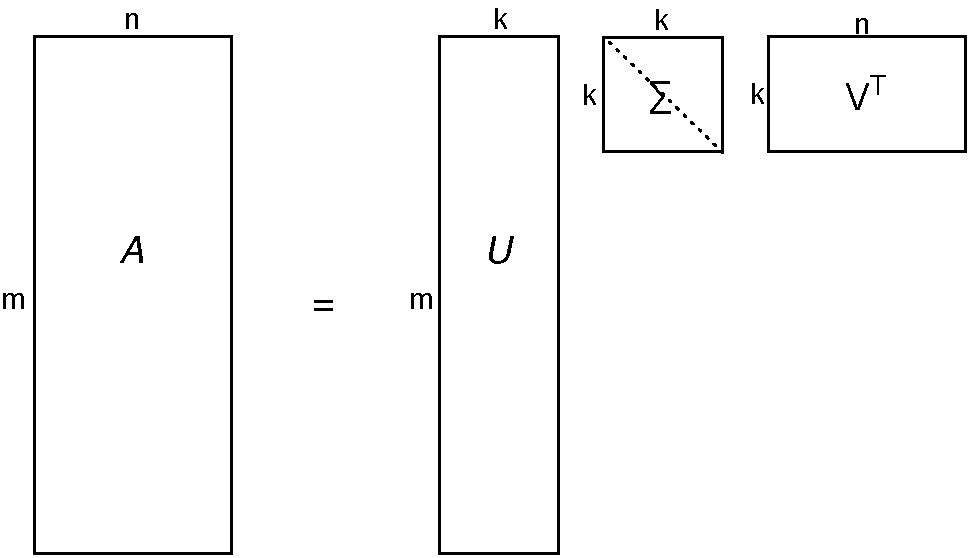
\includegraphics[width=\textwidth]{figures/svd_figure}
    \end{center}
    \caption{Singular Value Decomposition}
    \label{fig:svd}
\end{figure}

\begin{enumerate}
    \item With the cross product matrix, $A^TA$ and $AA^T$
    \item With the cyclic matrix $H(A) =
        \begin{bmatrix}
            0   & A\\
            A^* & 0
        \end{bmatrix}$
\end{enumerate}

The singular values are the nonnegative square roots of the eigenvalues of the
cross product matrix. This approach may imply a severe loss of accuracy in the
smallest singular values. The cyclic matrix approach is an alternative that
avoids this problem, but at the expense of significantly increasing the cost of
the computation.

Computing the cross product matrix explicitly is not recommended, especially in
the case of sparse A. Bidiagonalization was proposed by Golub and
Kahan~\cite{golub1965} as a way of tridiagonalizing the cross product matrix
without forming it explicitly.

Consider the following decomposition
\begin{gather*}
    A = P B Q^T,
\end{gather*}

where P and Q are unitary matrices and B is an $m\times n$ upper bidiagonal
matrix. Then the tridiagonal matrix $BB^T$ is unitarily similar to $AA^T$.
Additionally, specific methods exist that compute the singular values of $B$
without forming $BB^T$. Therefore, after computing the SVD of B,
\begin{gather*}
    B = X \Sigma Y^T,
\end{gather*}
it only remains to compute the SVD of the original matrix with $U = PX$ and $V = QY$.

\section{Lanczos Bidiagonalization} % (fold)
\label{sec:lanczos_bidiagonalization}

The Lanczos algorithm is an iterative algorithm devised by Cornelius Lanczos
that is an adaptation of power methods to find eigenvalues and eigenvectors of a
square matrix or the singular value decomposition of a rectangular matrix. It is
particularly useful for finding decompositions of very large sparse matrices.

For a rectangular matrix $A$, the Lanczos bidiagonalization method computes a
sequence of Lanczos vectors $p_j \in \mathbb{R}^m$ and $q_j \in \mathbb{R}^n$
and scalars $\alpha_j$ and $\beta_j$ for $j = 1, 2, \ldots, k$ as follows:

\begin{algorithm}[Lanczos Bidiagonalization Algorithm]
 % \label{alg:lanczos-bidiagonalization}
\begin{algorithmic}[1]
     \State Choose a unit-norm vector $q_1$ and let $\beta_0 = 0$ and $p_0 = 0$
     \For{$j = 1, 2, \ldots, k$}
        \State $p_j \set Aq_j - \beta_{j-1} p_{j-1}$
        \State $\alpha_j \set \vectornorm{p_j}_2$
        \State $p_j \set p_j/\alpha_j$
        \State $q_{j+1} \set A^Tp_j - \alpha_j q_j$
        \State $\beta_j \set \vectornorm{q_{j+1}}_2$
        \State $q_{j+1} \set q_{j+1}/\beta_j$
    \EndFor
\end{algorithmic}
\end{algorithm}


After $k$ steps, we can generate the bidiagonal matrix $B_k$ as follows,
\[
\begin{bmatrix}
    \alpha_1    & \beta_1   &           &           &               & \\
                & \alpha_2  & \beta_2   &           &               & \\
                &           & \alpha_3  & \beta_3   &               & \\
                &           &           & \ddots    & \ddots        & \\
                &           &           &           & \alpha_{k-1}  & \beta_{k-1} \\
                &           &           &           &               & \alpha_k
\end{bmatrix}
\]
In exact arithmetic the Lanczos vectors are orthonormal such that,
\begin{gather*}
    P_{k+1} = (p_1, p_2, \dotsc, p_{k+1}) \in \mathbb{R}^{m \times (k+1)},
        P_{k+1}^T P_{k+1} = I_{k+1} \\
    Q_{k+1} = (q_1, q_2, \dotsc, q_{k+1}) \in \mathbb{R}^{n \times  (k+1)},
        Q_{k+1}^T Q_{k+1} = I_{k+1}.
\end{gather*}

\begin{figure}[tb]
    \centering
        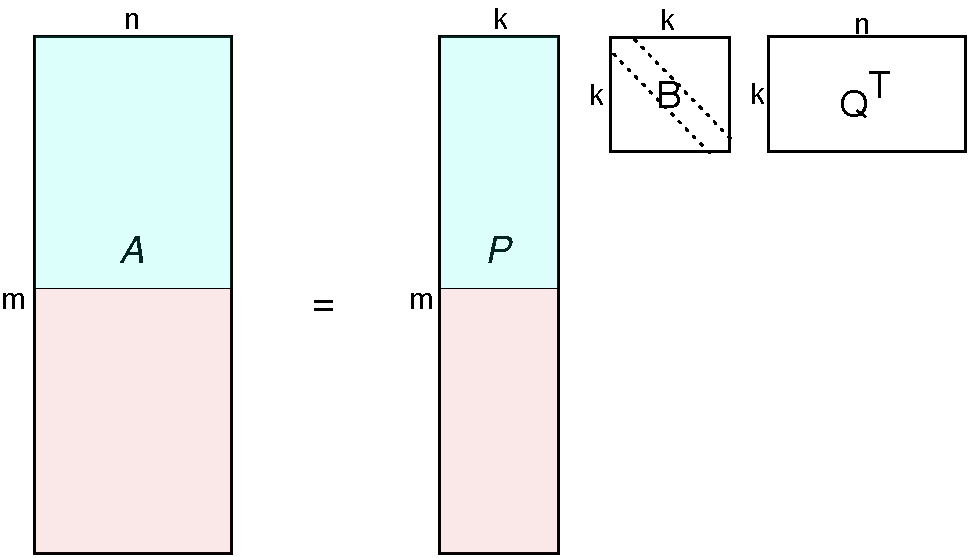
\includegraphics[width=\textwidth]{figures/lanczos_bidiag_segment}
    \caption{Lanczos bidiagonalization of $A$}
    \label{fig:lanczos}
\end{figure}
After $k$ Lanczos steps, the Ritz values $\tilde{\sigma_i}$ (approximate singular
values of A) are equal to the computed singular values of $B_k$, and the
Ritz vectors are
\begin{gather*}
    \tilde{u_i} = P_k x_i,  \qquad  \tilde{v_i} = Q_k y_i
\end{gather*}
% subsubsection lanczos_bidiagonalization (end)

\section{Dealing with Loss of Orthogonality} % (fold)
\label{sec:dealing_with_loss_of_orthogonality}

After a sufficient number of steps the Lanczos vectors start to lose their
mutual orthogonality, and this happens together with the appearance in the
spectrum of $B_j$ of repeated and spurious Ritz values. The simplest cure for
this loss of orthogonality is full orthogonalization. In Lanczos
bidiagonalization, two sets of Lanczos vectors are computed, so full
orthogonalization amounts to orthogonalizing vector $p_j$ explicitly with
respect to all the previously computed left Lanczos vectors, and orthogonalizing
vector $q_{j+1}$ explicitly with respect to all the previously computed right
Lanczos vectors.

\begin{algorithm}[Lanczos Bidiagonalization with Partial Reorthogonalization]
% \label{alg:one-sided_lanczos}
\begin{algorithmic}[1]
     \State Choose a unit-norm vector $q_1$ and let $\beta_0 = 0$ and $p_0 = 0$
     \For{$j = 1, 2, \ldots, k$}
        \State $p_j \set Aq_j - \beta_{j-1} p_{j-1}$
        \State $\alpha_j \set \vectornorm{p_j}_2$
        \State $p_j \set p_j/\alpha_j$
        \State $q_{j+1} \set A^Tp_j - \alpha_j q_j$
        \State Orthogonalize $q_{j+1}$ with respect to $Q_j$
        \State $\beta_j \set \vectornorm{q_{j+1}}_2$
        \State $q_{j+1} \set q_{j+1}/\beta_j$
    \EndFor
\end{algorithmic}
\end{algorithm}

There is a variation of this orthogonalization that maintains the effectiveness
of full reorthogonalization but with a considerably reduced cost. This technique
was proposed by Simon and Zha~\cite{simon2000}. The idea comes from the observation that,
in the Lanczos bidiagonalization procedure without reorthogonalization, the
level of orthogonality of left and right Lanczos vectors go hand in hand. This
observation led to Simon and Zha to propose what they called the one-sided version
shown in Algorithm~2. %\ref{alg:one-sided_lanczos}.
% section dealing_with_loss_of_orthogonality (end)

\section{Enhancements for Distributed Efficiency} % (fold)
\label{sec:parallelizing}

\begin{algorithm}[Distributed version of Lanczos BPRO]% \label{alg:one-sided_lanczos}
\begin{algorithmic}[1]
     \State Choose a unit-norm vector $q_1$ and let $\beta_0 = 0$ and $p_0 = 0$
     \For{$j = 1, 2, \ldots, k$}
        \Statex {\footnotesize Transition step}
        \State $p_j \set Aq_j - \beta_{j-1} p_{j-1}$
        \State $\alpha_j \set \vectornorm{p_j}_2^2$   \Comment Delayed normalization
        \State $q_{j+1} \set A^Tp_j - \alpha_j q_j$
        \Statex {\footnotesize Merge step}
        \State Concatenate $p_j$ across parallel segments
        \State Sum $q_{j+1}$ across parallel segments
        \Statex {\footnotesize Final Step}
        \State $\alpha_j \set \sqrt{\alpha_j}$
        \State $p_j \set p_j/\alpha_j$
        \State $q_j \set q_j/\alpha_j$
        \State Orthogonalize $q_{j+1}$ with respect to $Q_j$
        \State $\beta_j \set \vectornorm{q_{j+1}}_2$
        \State $q_{j+1} \set q_{j+1}/\beta_j$
    \EndFor
\end{algorithmic}
\end{algorithm}

% section parallelizing (end)

% When using TeXShop on the Mac, let it know the root document. The following must be one of the first 20 lines.
!TEX root = ../design.tex

\chapter[Regression]{Regression}
\begin{moduleinfo}
\item[History]
	\begin{modulehistory}
		\item[v0.1] Initial version, including background of regression
	\end{modulehistory}
\end{moduleinfo}

% Abstract. What is the problem we want to solve?

Regression analysis is a statistical tool for the investigation of
relationships between variables. Usually, the investigator seeks to ascertain
the causal effect of one variable upon another—the effect of a price increase
upon demand, for example, or the effect of changes in the money supply upon the
inflation rate. More specifically, regression analysis helps one understand how
the typical value of the dependent variable changes when any one of the
independent variables is varied, while the other independent variables are held
fixed.

Regression models involve the following variables:
\begin{enumerate}
    \item The unknown parameters, denoted as $\beta$, which may represent a scalar or a vector.
    \item The independent variables, $x$
    \item The dependent variables, $y$
\end{enumerate}

\section{Linear Methods for Regression} % (fold)
\label{sub:linear_methods_for_regression}

% subsection linear_methods_for_regression (end)

\section{Regularization} % (fold)
\label{sub:regularization}

Usually, $y$ is the result of measurements contaminated by small errors
(noise). Frequently, ill-conditioned or singular systems also arise in the iterative solution of nonlinear systems or optimization problems. In all such situations, the vector $x = {A}^{-1}y$ (or in the full rank overdetermined
case $A^+ y$, with the pseudo inverse $A^+ = (A^T A)^{−1}A^T X)$, if it exists at all, is usually a meaningless bad approximation to x.

Regularization techniques are needed to obtain meaningful solution estimates 
for such ill-posed problems, and in particular when the number of parameters 
is larger than the number of available measurements, so that standard least 
squares techniques break down.

\subsection{Linear Ridge Regression}
Ridge regression is the most commonly used method of regularization of
ill-posed problems. Mathematically, it seeks to minimize

\begin{equation}
Q\left(\vec{w},w_0;\lambda\right)\equiv \min_{\vec{w},w_0}\left[ \frac{1}{2N} \sum_{i=1}^{N} \left( y_i - w_0 -
    \vec{w} \cdot \vec{x}_i \right)^2
  +\frac{\lambda}{2}\|\vec{w}\|_2^2 \right]\ ,
\end{equation}
for a given value of $\lambda$, where $\vec{w}$ and $w_0$ are the fitting coefficients, and $\lambda$
is a non-negative regularization parameter. $\vec{w}$ is a vector in
$d$ dimensional space, and
\begin{equation}
\|\vec{w}\|_2^2 = \sum_{j=1}^{d}w_j^2 = \vec{w}^T\vec{w}\ .
\end{equation}
When $\lambda = 0$, $Q$ is
the mean squared error of the fitting.

The intercept term $w_0$ is not regularized, because this term is
fully decided by the mean values of $y_i$ and $\vec{x}_i$ and the
values of $\vec{w}$, and does not affect the model's complexity.

$Q\left(\vec{w},w_0;\lambda)$ is a quadratic function of $\vec{w}$ and
  $w_0$, and thus can be solved analytically
\begin{equation}
\vec{w}_{ridge}=\left(\lambda\vec{I}_d +
  \vec{X}^T\vec{X}\right)^{-1}\vec{X}^T\vec{y}\ .
\end{equation}
By using the available Newton method (Sec. 6.2.4), the above quantity can be easily
calculated from one single step of the Newton method.

Many packages for Ridge regularization actually regularize the fitting
coefficients not for the fitting model for the original data but for
the data that has be scaled. MADlib also provides this option. When
the normalization parameter is set to be True, which is by default
False, the data will be first converted to the following before
applying the Ridge regularization.
\begin{equation}
  x_i' \leftarrow \frac{x_i - \langle x_i \rangle}{\langle (x_i -
    \langle x_i \rangle)^2\rangle} \ ,
\end{equation}
\begin{equation}
y_i \leftarrow y_i - \langle y_i \rangle \ ,
\end{equation}
where $\langle \cdot \rangle = \sum_{i=1}^{N} \cdot / N$.

Note that Ridge regressions for scaled data and un-scaled data are not equivalent.

\subsection{Elastic Net Regularization} % (fold)
\label{ssub:elastic_net_regularization}
As a continuous shrinkage method, ridge regression achieves its better prediction performance through a bias–variance trade-off. However, ridge regression cannot produce a parsimonious model, for it always keeps all the predictors in the model~\cite{zou2005}. Best subset selection in contrast produces a sparse model, but it is extremely variable because of its inherent discreteness. 

A promising technique called the lasso was proposed by Tibshirani (1996). The 
lasso is a penalized least squares method imposing an L1-penalty on the 
regression coefficients. Owing to the nature of the L1-penalty, the lasso does 
both continuous shrinkage and automatic variable selection simultaneously.
 
Although the lasso has shown success in many situations, it has some 
limitations. Consider the following three scenarios: 
\begin{enumerate}
    \item In the Number of features ($p$) >> Number of observations ($n$) case, the lasso selects at most $n$ variables before it saturates, because of the nature of the convex optimization problem. This seems to be a limiting feature for a variable selection method. Moreover, the lasso is not well defined unless the bound on the $L_1$-norm of the coefficients is smaller than a certain value.
    \item If there is a group of variables among which the pairwise correlations are very high, then the lasso tends to select only one variable from the group and does not care which one is selected.
    \item For usual n>p situations, if there are high correlations between predictors, it has been empirically observed that the prediction performance of the lasso is dominated by ridge regression. 
\end{enumerate}

These scenarios make lasso an inappropriate variable selection method in some situations. 

Hui Zou and Trevor Hastie [42] introduce a new regularization 
technique called the 'elastic net'. Similar to the lasso, the elastic net 
simultaneously does automatic variable selection and continuous
shrinkage, and it can select groups of correlated variables. It is like a 
stretchable fishing net that retains `all the big fish'.

The elastic net regularization minimizes the following target function
\begin{equation} \label{eq:target}
\min_{\vec{w} \in R^N}L(\vec{w}) + \lambda \left[\frac{1-\alpha}{2}\|\vec{w}\|_2^2 +
  \lambda\alpha \|\vec{w}\|_1\right]\ ,
\end{equation}  
where $\|\vec{w}\|_1 = \sum_{i=1}^N|w_i|$ and $N$ is the number of features.

For the elastic net regularization on linear models, 
\begin{equation}
L(\vec{w}) = \frac{1}{2M}\sum_{m=1}^M\left(y_m - w_0 - \vec{w} \cdot
  \vec{x}_m\right)^2\ ,
\end{equation}
where the sum is over all observations and $M$ is the total number of
observation.

For the elastic net regularization on logistic models,
\begin{equation}
L(\vec{w}) = \sum_{m=1}^M\left[y_m \log\left(1 + e^{-(w_0 +
      \vec{w}\cdot\vec{x}_m)}\right) + (1-y_m) \log\left(1 + e^{w_0 +
      \vec{w}\cdot\vec{x}_m}\right)\right]\ ,
\end{equation}
where $y_m \in \{0,1\}$.

\subsubsection{Optimizer Algorithms}
Right now, we support two algorithms for optimizer. The default one is
FISTA, and the other is IGD.

\paragraph{FISTA}

Fast Iterative Shrinkage Thresholding Algorithm (FISTA) with {\bf
  backtracking step size} [4]:
\vspace{0.2in}
\hline
\vspace{0.2in}
{\bf Step $0$}: Choose $\delta>0$ and $\eta > 1$, and
$\vec{w}^{(0)} \in R^N$. Set $\vec{v}^{(1)}=\vec{w}^{(0)}$ and
$t_1=1$.

{\bf Step $k$}: ($k \ge 1$) Find the smallest nonnegative integers
$i_k$ such that with $\bar{\delta} = \delta_{k-1}/\eta^{i_k-1}$
\begin{equation}
F(p_{\bar{\delta}}(\vec{v}^{(k)})) \le
Q_{\bar{\delta}}(p_{\bar{\delta}}(\vec{v}^{(k)}), \vec{v}^{k})\ .
\end{equation}
Set $\delta_k = \delta_{k-1}/\eta^{i_k-1}$ and compute
\begin{equation}
\vec{w}^{(k)}  =  p_{\delta_k}\left(\vec{v}^{(k)}\right)\ , 
\end{equation}
\begin{equation}
t_{k+1} = \frac{1 + \sqrt{1 + 4t_k^2}}{2}\ ,
\end{equation}
\begin{equation}
\vec{v}^{(k+1)} = \vec{w}^{(k)} +
\frac{t_k-1}{t_{k+1}}\left(\vec{w}^{(k)} - \vec{w}^{(k-1)}\right)\ .
\end{equation}
\vspace{0.2in}
\hline
\vspace{0.2in}
Here,
\begin{equation}
F(\vec{w}) = f(\vec{w}) + g(\vec{w})\ ,
\end{equation}
where $f(\vec{w})$ is the differentiable part of
Eq. (\ref{eq:target}) and $g(\vec{w})$ is the non-differentiable part. For linear models, 
\begin{equation}
f(\vec{w}) = \frac{1}{2M}\sum_{m=1}^M\left(y_m - w_0 - \vec{w} \cdot
  \vec{x}_m\right)^2 + \frac{\lambda(1-\alpha)}{2}\|\vec{w}\|_2^2\ ,
\end{equation}
and for logistic models,
\begin{equation}
f(\vec{w}) = \sum_{m=1}^M\left[y_m \log\left(1 + e^{-(w_0 +
      \vec{w}\cdot\vec{x}_m)}\right) + (1-y_m) \log\left(1 + e^{w_0 +
      \vec{w}\cdot\vec{x}_m}\right)\right] + \frac{\lambda(1-\alpha)}{2}\|\vec{w}\|_2^2\ .
\end{equation}
And for both types of models, 
\begin{equation}
g(\vec{w}) = \lambda\alpha\sum_{i=1}^N|w_i|\ .
\end{equation}

And 
\begin{equation}
Q_{\delta}(\vec{a}, \vec{b}) := f(\vec{b}) + \langle \vec{a} -
\vec{b}, \nabla f(\vec{b})\rangle + 
\frac{1}{2\delta}\|\vec{a} - \vec{b}\|^2 + g(\vec{a})\ ,
\end{equation}
where $\langle\cdot\rangle$ is just the usual vector dot product.

And the proxy function is defined as
\begin{equation}
p_\delta (\vec{v}) := \underset{\vec{w}}{\operatorname{arg\,min}} \left[g(\vec{w}) +
  \frac{1}{2\delta}\left\|\vec{w} - \left(\vec{v} - \delta\,\nabla f(\vec{v})\right)\right\|^2  \right]
\end{equation}
For our case, where $g(\vec{w}) = \lambda\alpha\sum_{i=1}^N|w_i|$, the
proxy function is simply equal to the soft-thresholding function
\begin{equation}
p_\delta (v_i) = \left\{ \begin{array}{ll}
v_i - \lambda\alpha\delta u_i\ , \quad  & \mbox{if } v_i > \lambda\alpha\delta
u_i \\
0\ , \quad & \mbox{otherwise} \\
v_i + \lambda\alpha\delta u_i\ , \quad & \mbox{if } v_i < - \lambda\alpha\delta u_i
\end{array}
\right.
\end{equation}
where 
\begin{equation}
\vec{u} = \vec{v} - \delta\,\nabla f(\vec{v})\ .
\end{equation}

{\bf Active set method} is used in our implementation for FISTA to
speed up the computation. Considerable speedup is obtained by
organizing the iterations around the active set of features— those
with nonzero coefficients. After a complete cycle through all the
variables, we iterate on only the active set till convergence. If
another complete cycle does not change the active set, we are done,
otherwise the process is repeated.

{\bf Warm-up method} is also used to speed up the computation. When
the option parameter $warmup$ is set to be $True$, a series of lambda
values, which is strictly descent and ends at the lambda value that
the user wants to calculate, will be used. The larger lambda gives
very sparse solution, and the sparse solution again is used as the
initial guess for the next lambda's solution, which will speed up the
computation for the next lambda. For larger data sets, this can
sometimes accelerate the whole computation and might be faster than
computation on only one lambda value.

{\bf Note:} Our implementation is a little bit different from the
original FISTA. In the original FISTA, during the backtracking
procedure, the algorithm is searching for a non-negative integer $i_k$
and the new step size is $\delta_k = \delta_{k-1}/\eta^{i_k}$. Thus
the step size is non-increasing. Here, we allow the step size to
increase by using $\delta_k = \delta_{k-1}/\eta^{i_k-1}$ so that
larger step sizes can be tried by the algorithm. Tests show that this
is actually faster.

\paragraph{IGD}

The Incremental Gradient Descent (IGD) algorithm is a stochastic
algorithm by its nature. So it is difficult to get sparse
solutions. What we implemented is Stochastic Mirror Descent Algorithm
made Sparse (SMIDAS). The inverse p-form link function is used
\begin{equation} \label{eq:f}
h_j^{-1}(\vec{\theta}) = \frac{\mbox{sign}(\theta_j)\vert \theta_j
  \vert^{p-1}}{\|\theta\|_p^{p-2}}\ ,
\end{equation}
where
\begin{equation}
\|\theta\|_p = \left(\sum_j \vert \theta \vert ^p\right)^{1/p}\ ,
\end{equation}
and $\mbox{sign}(0) = 0$.
\vspace{0.2in}
\hline
\vspace{0.2in}
Choose step size $\delta > 0$.

Let $p = 2\log d$ and let $h^{-1}$ be as in Eq. (\ref{eq:f})

Let $\vec{\theta} = \vec{0}$

{\bf for} $k = 1,2,\dots$

\quad $\vec{w} = h^{-1}(\vec{\theta})$

\quad $\vec{v} = \nabla f(\vec{w})$

\quad $\tilde{\vec{\theta}} = \theta - \delta \, \vec{v}$

\quad $\forall j, \theta_j = \mbox{sign}(\tilde{\theta}_j)\max (0,
\vert \tilde{\theta}_j \vert- \lambda\alpha\delta)$
\vspace{0.2in}
\hline
\vspace{0.2in}

The resulting fitting coefficients of this algorithm is not really
sparse, but the values are very small (usually $< 10^{15}$), which can
be safely set to be zero after filtering with a threshold.

This is done as the following: (1) multiply each coefficient with the
standard deviation of the corresponding feature (2) compute the
average of absolute values of re-scaled coefficients (3) divide each
rescaled coefficients with the average, and if the resulting absolute
value is smaller than <em>threshold</em>, set the original coefficient
to be zero.

IGD is in nature a sequential algorithm, and when running in a
distributed way, each segment of the data runs its own SGD model, and
the models are averaged to get a model for each iteration. This
average might slow down the convergence speed, although we acquire the
ability to process large data set on multiple machines. So this
algorithm provides an option <em>parallel</em> to let the user choose
whether to do parallel computation.

IGD also implements the {\bf warm-up method}.

{\bf Stopping Criteria} Both {\bf FISTA} and {\bf IGD} compute the average difference
between the coefficients of two consecutive iterations, and if the
difference is smaller than <em>tolerance</em> or the iteration number
is larger than <em>max_iter</em>, the computation stops.


% subsubsection elastic_net_regularization (end)
% subsection regularization (end)

% When using TeXShop on the Mac, let it know the root document. The following must be one of the first 20 lines.
% !TEX root = ../design.tex

\chapter[Clustering (k-means et al.)]{Clustering ($k$-Means et al.)}

\begin{moduleinfo}
\item[Author] \href{mailto:Florian.Schoppmann@emc.com}{Florian Schoppmann} (version 0.5 only)
\item[History]
	\begin{modulehistory}
		\item[v0.5] Initial revision of design document, complete rewrite of module, arbitrary user-specifyable distance and recentering functions
		\item[v0.3] Multiple seedings methods (kmeans++, random, user-specified list of centroids), multiple distance functions (corresponding recentering function hard-coded), simplified silhouette coefficient as goodness-of-fit measure
		\item[v0.1] Initial version, always use kmeans++ for seeding
	\end{modulehistory}
\end{moduleinfo}


% Abstract. What is the problem we want to solve?
Clustering refers to the problem of partitioning a set of objects into homogeneous subsets, i.e., such that objects in the same group have \emph{similar} properties. Arguably the best-known clustering problem is \emph{$k$-means}. Here, one is given $n$ points $x_1, \dots, x_n \in \R^d$, and the goal is to position $k$ centroids $c_1, \dots, c_k \in \R^d$ so that the sum of squared Euclidean distances between each point and its closest centroid is minimized. A cluster is identified by its centroid and consists of all points for which this centroid is closest. Formally, we wish to minimize the following objective function:
\begin{gather*}
    (c_1, \dots, c_k) \mapsto \sum_{i=1}^n \min_{j=1}^k \dist(x_i, c_j) \SiM,
\end{gather*}
where $\dist(x,y) := \| x - y \|_2^2$. A straightforward generalization of the above minimization problem is to choose a different metric $\dist$. Strictly speaking, this is no longer $k$-means; for instance, choosing $\dist(x,y) = \| x - y\|_1$ yields the $k$-median problem instead.

Despite certain reservations, we follow the practice of many authors and use ``$k$-means'' also to refer to a particular algorithm (as opposed to an optimization problem), as discussed below.

\section{Overview of Algorithms} \label{sec:kmeans:Algorithms}

% Explain the algorithm at a high-level -- do not talk about specific variations or implementation details. Give some theoretical background: Is the problem hard? What results can we expect?
The $k$-means problem is NP-hard in general Euclidean space (even for just two clusters) \cite{ADH09a} and for a general number of clusters (even in the plane) \cite{MNV10a}. However, the local-search heuristic proposed by \citeauthor{L82a}~\cite{L82a} performs reasonably well in practice. In fact, it is so ubiquitous today that it is often referred to as the standard algorithm or even just the $k$-means algorithm. At a high level, it works as follows:

\begin{enumerate}
	\item Seeding phase: Find initial positions for $k$ centroids $c_1, \dots, c_k$.
	\item Assign each point $x_1, \dots, x_n$ to its closest centroid. \label{enum:kmeans_abstract_points}
	\item Move each centroid $c$ to a position that minimizes the sum of distances between $c$ and each point assigned to $c$. (Note that if ``distance'' refers to the squared Euclidean distance, then this position is the barycenter/mean of all points assigned to $c$.)
	\item If convergence has been reached, stop. Otherwise, goto \eqref{enum:kmeans_abstract_points}.
\end{enumerate}

Since the value of the objective function decreases in every step, and there are only finitely many clusterings, the algorithm is guaranteed to converge to a local minimum \cite[Section~16.4]{CS08a}. While it is known that there are instances for which \citeauthor{L82a}'s heuristic takes exponentially many steps~\cite{V09a}, it has been shown that the algorithm has polynomial smoothed complexity \cite{AMR09a}---thus giving some theoretical explanation for good results in practice. With a clever seeding technique, \citeauthor{L82a}'s heuristic is moreover $O(\log k)$-competitive \cite{AV07a}.


\subsection{Algorithm Variants}

% Give an overview and references to variations that exist for this algorithm.
\paragraph{Seeding}

The quality of $k$-means is highly influenced by the choice of the seeding \cite{AV07a}. The following is a non-exhaustive list of options:
\begin{enumerate}
	\item Manual: User-specified list of initial centroid positions.
	\item Uniformly at random: Choose the $k$ centroids uniformly at random among the point set
	\item \texttt{$k$-means++}: Perform seeding so that the objective function is minimized in expectation \cite{AV07a}
	\item Use a different clustering algorithm for determining the seeding \cite{MNU00a}
	\item Run $k$-means with multiple seedings and choose the clustering with lowest cost
\end{enumerate}

\paragraph{Repositioning}

Most $k$-means formulations in textbooks do not detail the case where a centroid has no points assigned to it. It is an easy observation that moving a stray centroid in this case can only decrease the objective function. This can be done in a simple way (move onto a random point) or more carefully (e.g., move so that the objective function is minimized in expectation).

\paragraph{Convergence Criterion}

There are several reasonable convergence criteria. E.g., stop when:
\begin{enumerate}
	\item The number of repositioned centroids is below a given threshold
	\item The change in the objective drops below a given threshold
	\item The maximum number of iterations has been reached
	\item See, e.g., \textcite[Section~16.4]{CS08a} for more options.
\end{enumerate}

\paragraph{Variable Number of Clusters}

The number of clusters $k$ could be determined by the seeding algorithm (instead of being a parameter) \cite{MNU00a}. Strictly speaking, however, the algorithm should not be called $k$-means in this case.


\section{Seeding Algorithms}

In the following, we describe the seeding methods to be implemented for MADlib.

\subsection{Uniform-at-random Sampling}

Uniform-at-random sampling just uses the algorithms described in Section~\ref{sec:SampingWOReplacement}.

\subsection[k-means++]{$k$-means++}

\texttt{$k$-means++} seeding \cite{AV07a} starts with a single centroid chosen randomly among the input points. It then iteratively chooses new centroids from the input points until there are a total of $k$ centroids. The probability for picking a particular point is proportional to its minimum distance to any existing centroid. Intuitively, \texttt{$k$-means++} favors seedings where centroids are spread out over the whole range of the input points, while at the same time not being too susceptible to outliers.

\subsubsection{Formal Description}

\begin{algorithm}[$k$-means++$(k, P, \dist, C)$] \label{alg:kmeans++}
\alginput{Number of desired centroids $k$, set $P$ of points in $\R^d$, metric $\dist$, \\
	set $C$ of initial centroids}
\algoutput{Set of centroids $C$}
\begin{algorithmic}[1]
	\If{$C = \emptyset$}
		\State $C \set \{ \text{initial centroid chosen uniformly at random from } P \}$ \label{alg:kmeanspp:firstCentroid}
	\EndIf
	\While{$|C| < k$} \label{alg:kmeans++:for}
		\State $C \set C \cup \{ \text{random $p \in P$ with probability proportional to }\min_{c \in C} \dist(p,c) \}$ \label{alg:kmeanspp:nextcentroid}
	\EndWhile
\end{algorithmic}
\end{algorithm}

\begin{description}
	\item[Runtime] A naive implementation needs $\Theta(k^2 n)$ distance calculations, where $n = |P|$. A single distance calculation takes $O(d)$ time.
	\item[Space] Store $k$ centroids.
	\item[Subproblems]
		The existing \ref{sym:weighted_sample} subroutine can be used for:
		\begin{itemize}
			\item Line~\ref{alg:kmeanspp:firstCentroid}: Sample uniformly at random
			\item Line~\ref{alg:kmeanspp:nextcentroid}: Sample according to a discrete probability distribution.
		\end{itemize}
\end{description}

The number of distance calculations could be reduced by a factor of $k$ if we store, for each point $p \in P$, the distance to its closest centroid. Then, each iteration only needs $n$ distance calculations (i.e., only between the most recently added centroid and all points). In total, these are $\Theta(k n)$ distance calculations. Making this idea explicit leads to the following algorithm.

\begin{algorithm}[$k$-means++-ext$(k, P, \dist)$] \label{alg:kmeans++ext}
\alginput{Number of desired centroids $k$, set $P$ of points in $\R^d$, metric $\dist$, \\
	set $C$ of initial centroids}
\algoutput{Set of centroids $C$}
\algprecond{For all $p \in P: \delta[p] = \min_{c \in C} \dist(p, c)$ (or $\delta[p] = \infty$ if $C = \emptyset$)}
\begin{algorithmic}[1]
	\While{$|C| < k$} \label{alg:kmeans++ext:for}
		\State $\mathit{lastCentroid} \set \ref{sym:weighted_sample}(P, \delta)$ \label{alg:kmeans++ext:nextCentroid} \Comment{$\delta$ denotes the mapping $p \mapsto \delta[p]$}
		\State $C \set C \cup \{ \mathit{lastCentroid} \}$
		\For{$p \in P$} \label{alg:kmeans++ext:pointLoop}
			\If{$\dist(p, \mathit{lastCentroid}) < \delta[p]$}
				\State $\delta[p] \set \dist(p, \mathit{lastCentroid})$
			\EndIf
		\EndFor
	\EndWhile
\end{algorithmic}
\end{algorithm}

\begin{description}
	\item[Tuning] \label{kmeans++ext:tuning} The inner for-loop in line~\ref{alg:kmeans++ext:pointLoop} and \ref{sym:weighted_sample} in line~\ref{alg:kmeans++ext:nextCentroid} could be combined. With this improvement, only one pass over $P$ is necessary.
	\item[Runtime] $O(dkn)$ as explained before.
	\item[Space] Store $k$ centroids and $n$ distances.
	\item[Scalability] The outer while-loop is inherently sequential because the random variates in each iteration depend on all previous iterations. The inner loop, however, can be executed with data parallelism.
\end{description}

\subsubsection{Implementation as User-Defined Function}

In general, the performance benefit of explicitly storing points (i.e., choosing \ref{alg:kmeans++ext} over \ref{alg:kmeans++}) depends on the DBMS, the data, and the operating environment. The pattern of updating temporary state is made a bit more awkward in PostgreSQL due to its legacy of versioned storage. PostgreSQL performs an update by first inserting a new row and then marking the old row as invisible \cite[Section~23.1.2]{postgres:9.1.3}. As a result, for updates that touch many rows it is typically faster to copy the updated data into a new table (i.e., \texttt{CREATE TABLE AS SELECT} and \texttt{DROP TABLE}) rather than issue an \texttt{UPDATE}. Given these constraints, we currently choose to only implement algorithm~\ref{alg:kmeans++} (but not \ref{alg:kmeans++ext}) as the user-defined function \symlabel{kmeanspp\_seeding}{sym:kmeans++}.

\paragraph{In- and Output} The UDF expects the following arguments, and returns the following values:

\begin{center}
	\begin{tabularx}{\textwidth}{rlXl}
		\toprule%
		\textbf{Name} & \textbf{Description} & \textbf{Type}
		\\\otoprule
		In &
		\texttt{rel\_source} &
		Relation containing the points as rows &
		relation
		\\\midrule
		In &
		\texttt{expr\_point} &
		Point coordinates, i.e., the point $p$ &
		\specialcell{l}{expression\\ (floating-point vector)}
		\\\midrule
		In &
		\texttt{k} &
		Number of centroids &
		integer
		\\\midrule
		In &
		\texttt{fn\_dist} &
		Function returning the distance between two vectors &
		function
		\\\midrule
		In &
		\texttt{initial\_centroids} &
		Matrix containing the initial centroids as columns. This argument may be omitted (corresponding to an empty set $C$ of initial centroids). &
		floating-point matrix
		\\\midrule
		Out &
		&
		Matrix containing the $k$ centroids as columns &
		floating-point matrix
		\\\bottomrule
	\end{tabularx}
\end{center}

\paragraph{Components} The set of centroids $C$ is stored as a dense floating-point matrix that contains the centroids as columns vectors. Algoritm~\ref{alg:kmeans++} can be (roughly) translated into SQL as follow. We assume here that all function arguments are available as constants, and the matrix containing the centroids as columns is available as \texttt{centroids}. Line~\ref{alg:kmeanspp:firstCentroid} becomes:
\begin{lstlisting}[language=SQL,gobble=4]
    SELECT ARRAY[weighted_sample($expr_point, 1)]
    FROM $rel_source
\end{lstlisting}
Line~\ref{alg:kmeanspp:nextcentroid} is implemented using essentially the following SQL.
\begin{sql}[emph={centroids,fn_dist}]
    SELECT centroids || weighted_sample(
        $expr_point, (
            closest_column(
                centroids,
                $expr_point,
                fn_dist
        )).distance
    ) FROM $rel_source
\end{sql}
See Section~\ref{sec:matrix:closestColumn} for a description of \ref{sym:closestColumn}.

\subsubsection{Historical Implementations}

Implementation details and big-data heuristics that were used in previous versions of MADlib are documented here for completeness.

\begin{description}
	\item[v0.2.1beta and earlier] In lines~\ref{alg:kmeanspp:firstCentroid} and \ref{alg:kmeanspp:nextcentroid} of Algorithm~\ref{alg:kmeans++} use a random sample $P' \subsetneq P$.

		Here $P'$ will be a new random sample in each iteration. Under the a-priori assumption that a random point belongs to any of the $k$ (unknown) clusters with equal probability, sample enough points so that with high probability (e.g., $p = 0.999$) there is a point from each of the $k$ clusters.

		This is the classical occupancy problem (also called balls-into-bins model) \cite{F68a}: Throwing $r$ balls into $k$ bins, what is the probability that no bin is empty? The exact value is
		\begin{align*}
			u(r, k) = k^{-r} \sum_{i=0}^k (-1)^i \binom ki (k - i)^r
			\SiM.
		\end{align*}

		For $r,k \to \infty$ so that $r/k = O(1)$ we have the limiting form $u(r,k) \to (1 - e^{-r/k})^k =: \widetilde u(r, k)$. Rearranging $\widetilde u(r, k) > p$ gives $-\log(1 - \sqrt[k]p) \cdot k < r$. The smallest $r$ satisfying this inequality is chosen as the size of the sample set.
\end{description}

\section[Standard algorithm for k-means clustering]{Standard algorithm for $k$-means clustering}

The standard algorithm has been outlined in Section~\ref{sec:kmeans:Algorithms}. The formal description and our implementation are given below.

\subsection{Formal Description}

\begin{algorithm}[$k$-means$(k, P, \dist)$] \label{alg:kmeans}
\alginput{Set of initial centroids $C$, set $P$ of points, seeding strategy $\mathit{Seeding}$, metric $\dist$, \\
averaging function $\mathit{mean}$, convergence strategy $\mathit{Convergence}$}
\algoutput{Set $C$ of final means}
\algprecond{$i = 0$}
\begin{algorithmic}[1]
	\Repeat
		\State $i \set i + 1$
		\State $C_\text{old} \set C$
		\State $C \set \bigcup_{c \in C} \{ \mathit{mean} \{p \in P \mid \arg\min_{c' \in C} \dist(p, c') = c \} \}$ \label{alg:kmeans:MoveCentroids}
		\State $C \set \mathit{Seeding}(k, P, \dist, C)$ \label{alg:kmeans:Reseed} \Comment{Reseed ``lost'' centroids (if any)}
	\Until{$Convergence(C, C_\text{old}, P, i)$} \label{alg:kmeans:ConvergenceCond}
\end{algorithmic}
\end{algorithm}

\begin{description}
	\item[Runtime] See discussion in Section~\ref{sec:kmeans:Algorithms}.
	\item[Space] Store $2k$ centroids (both sets $C$ and $C_\text{old}$)
	\item[Scalability] The outer loop is inherently sequential. The recentering in line~\ref{alg:kmeans:MoveCentroids} is data-parallel (provided that the sets $C$ and $C_\text{old}$ are available on all computation nodes). Likewise, the convergence check in line~\ref{alg:kmeans:ConvergenceCond} is data-parallel if it only relies on distances between points $p$ and the set of centroids $C$, or the number of iterations.
\end{description}

\subsection{Implementation as User-Defined Function}

Algorithm~\ref{alg:kmeans} is implemented as the user-defined function \symlabel{kmeans}{sym:kmeans}. We choose to not make the convergence criterion a function argument but instead settle for parameters for the most typical criteria. Should the need arise, we might revoke that decision in the future. Moreover, the seeding strategy is currently not an argument, but \ref{sym:kmeans++} is always used in line~\ref{alg:kmeans:Reseed}.

\paragraph{In- and Output} The UDF expects the following arguments, and returns the following values:

\begin{center}
	\begin{tabularx}{\linewidth}{rlXl}
		\toprule%
		\textbf{Name} & \textbf{Description} & \textbf{Type}
		\\\otoprule
		In &
		\texttt{rel\_source} &
		Relation containing the points as tuples &
		relation
		\\\midrule
		In &
		\texttt{expr\_point} &
		Point coordinates, i.e., the point $p$ &
		\specialcell{l}{expression\\ (floating-point vector)}
		\\\midrule
		In &
		\texttt{initial\_centroids} &
		Matrix containing the initial centroids as columns &
		floating-point matrix
		\\\midrule
		In &
		\texttt{fn\_dist} &
		Function returning the distance between two vectors &
		function
		\\\midrule
		In &
		\texttt{agg\_centroid} &
		Aggregate returning the centroid for a set of points &
		function
		\\\midrule
		In &
		\texttt{max\_num\_iterations} &
		Convergence criterion: Maximum number of iterations &
		integer
		\\\midrule
		In &
		\texttt{min\_frac\_reassigned} &
		Convergence criterion: Convergence is reached if the fraction of points being reassigned to another centroid drops below \texttt{conv\_level} &
		floating-point
		\\\midrule
		Out & &
		Matrix containing the $k$ centroids as columns &
		floating-point matrix
		\\\bottomrule
	\end{tabularx}
\end{center}

\paragraph{Components}

The set of centroids $C$ is stored as a dense floating-point matrix that contains the centroids as columns vectors. Algoritm~\ref{alg:kmeans} can be (roughly) translated into SQL as follow. We assume here that all function arguments are available as constants, and the matrix containing the centroids is available as \texttt{centroids}. (These variables, which are unbound in the SQL statement, are shown in italic font.) Line~\ref{alg:kmeans:MoveCentroids} becomes:
%
\begin{sql}[emph={centroids,fn_dist}]
    SELECT matrix_agg(_centroid)
    FROM (
        SELECT $agg_centroid(_point) AS _centroid
        FROM (
            SELECT
                $expr_point AS _point,
                (closest_column(
                    centroids,
                    $expr_point,
                    fn_dist
                )).column_id AS _new_centroid_id
            FROM $rel_source
        ) AS _points_with_assignments
        GROUP BY _new_centroid_id
    ) AS _new_centroids
\end{sql}
See Section~\ref{sec:matrix:matrixAgg} for a description of \ref{sym:matrixAgg}.

It is a good idea to also compute the number of reassigned centroids, so that both line~\ref{alg:kmeans:MoveCentroids} and the convergence check in line~\ref{alg:kmeans:ConvergenceCond} can be computed with one pass over the data. To that end, we extend the inner-most query to also compute the previous closest centroid (i.e., we do a second \ref{sym:closestColumn} call where we pass matrix \texttt{old\_centroids} as first argument). During the aggregations in the two outer queries, we can then count (or sum up, respectively) the number of points that have been reassigned.

A caveat during testing whether a point has been reassigned is that centroid IDs are not constant over iterations: \ref{sym:closestColumn} returns a column index in the matrix \texttt{centroids}, and this matrix is the result of the \ref{sym:matrixAgg} aggregate---hence, the order of the columns is non-deterministic. We therefore cannot directly compare a column index from iteration $i$ to a column index from iteration $i - 1$, but instead need to translate the ``new'' index into an ``old'' index first. In order to do that, we extend the outermost query and also build up an array \texttt{old\_centroid\_ids}, where position $i$ will contain the column index that centroid $i$ had in the previous iteration. \Warning{A crucial assumption on the DBMS backend here is that the two aggregates \texttt{array\_agg} and \ref{sym:matrixAgg} see all tuples in the same order.} Putting everything together, the query becomes:
%
\begin{sql}[emph={centroids,old_centroids,old_centroid_ids,fn_dist}]
    SELECT
        matrix_agg(_centroid),        -- New value for: centroids
        array_agg(_new_centroid_id),  -- New value for: old_centroid_ids
        sum(_objective_fn),           -- New value for: objective_fn
        CAST(sum(_num_reassigned) AS DOUBLE PRECISION) / sum(_num_points) -- New value for: frac_reassigned
    FROM (
        SELECT
            (_new_centroid).column_id AS _new_centroid_id,
            sum((_new_centroid).distance) AS _objective_fn,
            count(*) AS _num_points,
            sum(
                CAST(old_centroid_ids[(_new_centroid).column_id + 1] != _old_centroid_id AS INTEGER)
            ) AS _num_reassigned,
            $agg_centroid(_point) AS _centroid
        FROM (
            SELECT
                $expr_point AS _point,
                closest_column(
                    centroids,
                    $expr_point,
                    fn_dist
                ) AS _new_centroid,
                (closest_column(
                    old_centroids,
                    $expr_point,
                    fn_dist
                )).column_id AS _old_centroid_id
            FROM $rel_source
        ) AS _points_with_assignments
        GROUP BY (_new_centroid).column_id
    ) AS _new_centroids
\end{sql}


Finally, line~\ref{alg:kmeans:Reseed} is simply implemented by calling function \ref{sym:kmeans++}. For a slight performance benefit, this function call should be guarded by a check if the number of centroids is lower than $k$.


% When using TeXShop on the Mac, let it know the root document.
% The following must be one of the first 20 lines.
% !TEX root = ../design.tex

\chapter[Convex Programming Framework]{Convex Programming Framework}
% Motivation. Why do we want to have this abstract layer?
The nature of MADlib drives itself to support many different kinds of data modeling modules, such as logistic regression, support vector machine, matrix factorization, etc.
However, keeping up with the state of the art and experimenting with individual data modeling modules require significant development and quality-assurance effort.
Therefore, to lower the bar of adding and maintaining new modules, it is crucial to identify the invariants among many important modules, in turn, abstract and encapsulate them as reusable components.

Bismarck \cite{DBLP:conf/sigmod/FengKRR12} is such a unified framework that links many useful statistical modeling modules and the relational DBMS, by introducing a well-studied formulation, convex programming, in between.
Incremental Gradient Descent (IGD) has also been shown as a very effective algorithm to solve convex programs in the relational DBMS environment.
But it is natural that IGD does not always fit the need of MADlib users who are applying convex statistical modeling to various domains.
Driven by this, convex programming framework in MADlib also implements other algorithms that solves convex programs, such as Newton's method and conjugate gradient methods.

\section{Introduction}
% Problem definition. What are the problems that we can solve, formally and example applications?
% linearly separable, unconstrained, continuous, deterministic, convex, minimization problems.
This section is to first explain, formally, the type of problems that we consider in MADlib convex programming framework, and then give a few example modules.

\subsection{Formulation}
We support numerical optimization problems with a objective function that is a sum of many component functions \cite{springerlink:10.1007/s10107-011-0472-0}, such as
\[\min_{w \in \mathbb{R}^N} \sum_{m=1}^M f_{z_m}(w),\]
where $z_m \in \mathcal{O}, m = 1,...,M,$ are observations, and $f_{z_m} : \mathbb{R}^N \mapsto \mathbb{R}$ are convex functions.
For simplicity, let $z_{1:M}$ denote $\{z_m \in \mathcal{O} | m = 1,...,M\}$.
Note: given $z_{1:M}$, let $F(w) = \sum_{m=1}^M f_{z_m}(w),$ and $F : \mathbb{R}^N \mapsto \mathbb{R}$ is also convex.

\subsection{Examples}
Many popular model can be formulated in the above form, with $f_{z_m}$ being properly specified.

\paragraph{Logistic Regression.} The component function is given by
\[f_{(x_m, y_m)}(w) = \log(1 + e^{- y_m w^{T} x_m}),\]
where $x_m \in \mathbb{R}^N$ are values of independent variables, and $y_m \in \mathbb{R}$ are values of the dependent variable, $m = 1,...,M.$

\paragraph{Linear SVM with hinge loss.} The component function is given by
\[f_{(x_m, y_m)}(w) = \max(0, 1 - y_m w^{T} x_m),\]
where $x_m \in \mathbb{R}^N$ are values of features, and $y_m \in \mathbb{R}$ are values of the label, $m = 1,...,M.$
Bertsekas \cite{springerlink:10.1007/s10107-011-0472-0} gives many other examples across application domains.

\section{Algorithms}
\paragraph{Gradient Descent.}
A most-frequently-mentioned algorithm that solves convex programs is gradient descent.
This is an iterative algorithm and the iteration is given by
\[w_{k+1} = w_k - \alpha_k \nabla F(w_k),\]
where, given $z_{1:M}$, $F(w) = \sum_{m=1}^M f_{z_m}(w),$ and $\alpha_k$ is a positive scalar, called stepsize (or step length).
Gradient descent algorithm is simple but usually recognized as a slow algorithm with linear convergence rate, while other algorithms like conjugate gradient methods and Newton's method has super-linear convergence rate \cite{nocedal2006numerical}.

\paragraph{Line Search Strategy}
% line search & trust region
Convex programming has been well studied in the past few decades, and two main classes of algorithms are widely considered: line search and trust region (\cite{nocedal2006numerical}, section 2.2).
Because line search is more commonly deployed and discussed, we focus on line search in MADlib, although some of the algorithms we discuss in this section can also easily be formulated as trust region strategy.
% general form of line search: w += \alpha p_k
All algorithms of line search strategies have the iteration given by
\[w_{k+1} = w_k + \alpha_k p_k,\]
where $p_k \in \mathbb{R}^N$ is search direction, and stepsize $\alpha_k$ \cite{nocedal2006numerical}.
Specifiedly, for gradient descent, $p_k$ is the steepest descent direction $- \nabla \sum_{m=1}^M f_{z_m}(w_k)$.

\subsection{Formal Description of Line Search}
\begin{algorithm}[line-search$(z_{1:M})$] \label{alg:line-search}
\alginput{Observation set $z_{1:M}$,\\
convergence criterion $\mathit{Convergence}()$,\\
start strategy $\mathit{Start}()$,\\
initialization strategy $\mathit{Initialization}()$,\\
transition strategy $\mathit{Transition}()$,\\
finalization strategy $\mathit{Finalization}()$}
\algoutput{Coefficients $w \in \mathbb{R}^N$}
\algprecond{$iteration = 0, k = 0$}
\begin{algorithmic}[1]
	\State $w_\text{new} \set \mathit{Start}(z_{1:M})$
	\Repeat
        \State $w_\text{old} \set w_\text{new}$
        \State $\mathit{state} \set \mathit{Initialization}(w_\text{new})$
		\For{$m \in 1..M$} \Comment{Single entry in the observation set}
			\State $\mathit{state} \set \mathit{Transition}(\mathit{state}, z_m)$
                \Comment{Usually computing derivative}
		\EndFor
		\State $w_\text{new} \set Finalization(\mathit{state})$
	\Until{$Convergence(w_\text{old}, w_\text{new}, \mathit{iteration})$}
    \State \Return $w_\text{new}$
\end{algorithmic}
\end{algorithm}

\paragraph{Programming Model.}
We above give the algorithm of generic line search strategy, in the fashion of the selected programming model supported by MADlib (mainly user-defined aggregate).

\paragraph{Parallelism.}
The outer loop is inherently sequential.
We require the inner loop is data-parallel.
Simple component-wise addition or model averaging \cite{DBLP:conf/nips/DuchiAW10} are used to merge two states.
A merge function is not explicitly added to the pseudocode for simplicity.
A separate discussion will be made when necessary.

\paragraph{Convergence criterion.}
Usually, following conditions are combined by AND, OR, or NOT.
\begin{enumerate}
    \item The change in the objective drops below a given threshold (E.g., negative log-likelihood, root-mean-square error).
    \item The value of the objective matches some pre-computed value.
    \item The maximum number of iterations has been reached.
    \item There could be more.
\end{enumerate}
In MADlib implementation, the computation of objective is paired up with line-search to share data I/O.

\paragraph{Start strategy.}
In most cases, zeros are used unless otherwise specified.

\paragraph{Transition and finalization strategies.}
The coefficients update code ($w_{k+1} \set w_k + \alpha_k p_k$) is put into either $\mathit{Transition}()$ or $\mathit{Finalization}()$.
These two functions contain most of the computation logic, for computing the search direction $p_k$.
We discuss details of individual algorithms in the following sections.
For simplicity, global iterator $k$ is read and updated in place by these functions without specifed as an additional argument.

\subsection{Incremental Gradient Descent (IGD)}
% motivation and introduction of IGD
A main challenge arises when we are handling large amount of data, $M >> 1,$ where the computation of $\nabla (\sum_{m=1}^M f_{z_m})$ requires a whole pass of the observation data which is usually expensive.
What distinguishes IGD from other algorithms is that it approximates  $\nabla (\sum_{m=1}^M f_{z_m}) = \sum_{m=1}^M (\nabla f_{z_m})$ by the gradient of a single component function $\nabla f_{z_m}$
\footnote{$z_m$ is usually selected in a stochastic fashion.
Therefore, IGD is also referred as stochastic gradient descent.
The convergence and convergence rate of IGD are well developed \cite{springerlink:10.1007/s10107-011-0472-0}, and IGD is often considered to be very effective with $M$ being very large \cite{DBLP:conf/nips/BottouB07}.}.
The reflection of this to the pseudocode makes the coefficients update code ($w_{k+1} \set w_k + \alpha_k p_k$) in $\mathit{Transition}()$ instead of in $\mathit{Finalization}()$.

\subsubsection{Initialization Strategy}
\begin{algorithm}[initialization-igd$(w)$] \label{alg:initialization-igd}
\alginput{Coefficients $w \in \mathbb{R}^N$}
\algoutput{Transition state $\mathit{state}$}
\begin{algorithmic}[1]
    \State $\mathit{state}.w_k \set w$
    \State \Return $\mathit{state}$
\end{algorithmic}
\end{algorithm}

\subsubsection{Transition Strategy}
\begin{algorithm}[transition-igd$(\mathit{state}, z_m)$] \label{alg:transition-igd}
\alginput{Transition state $\mathit{state}$,\\
observation entry $z_m$,\\
stepsize $\alpha \in \mathbb{R}^+$,\\
gradient function $\mathit{Gradient}()$}
\algoutput{Transition state $\mathit{state}$}
\begin{algorithmic}[1]
    \State $p_k \set - \mathit{Gradient}(\mathit{state}.w_k, z_m)$
        \Comment{Previously mentioned as $p_k = - \nabla f_{z_m}$}
    \State $\mathit{state}.w_{k+1} \set \mathit{state}.w_k + \alpha p_k$
    \State $k \set k + 1$
        \Comment{In-place update of the global iterator}
    \State \Return $\mathit{state}$
\end{algorithmic}
\end{algorithm}

\paragraph{Stepsize.}
In MADlib, we support only constant stepsize for simplicity.
Although IGD with constant stepsizes does not even have convergence guarantee \cite{springerlink:10.1007/s10107-011-0472-0}, but it works reasonably well in practice so far \cite{DBLP:conf/sigmod/FengKRR12} with some proper tuning.
Commonly-used algorithms to tune stepsize (\cite{bertsekas1999nonlinear}, appendix C) are mostly heuristics and do not have strong guarantees on convergence rate.
More importantly, these algorithms require many evaluations of the objective function, which is usually very costly in use cases of MADlib.

\paragraph{Gradient function.}
A function where IGD accepts computational logic of specified modules.
In MADlib convex programming framework, currently, there is no support of objective functions that does not have gradient or subgradient.

\subsubsection{Finalization Strategy}
\begin{algorithm}[finalization-igd$(\mathit{state})$] \label{alg:finalization-igd}
\alginput{Transition state $\mathit{state}$}
\algoutput{Coefficients $w \in \mathbb{R}^N$}
\begin{algorithmic}[1]
    \State \Return $\mathit{state}.w_k$
        \Comment{Trivially return $w_k$}
\end{algorithmic}
\end{algorithm}

\subsection{Conjugate Gradient Methods}
% Simple description of conjugate gradient
Conjugate gradient methods that solve convex programs are usually refered as nonlinear conjugate gradient mthods.
The key difference between conjugate gradient methods and gradient descent is that conjuagte gradient methods perform adjustment of the search direction $p_k$ by considering gradient directions of previous iterations in some intriguing way.
We skip the formal desciption of conjugate gradient methods that can be found in the references (such as Nocedal \& Wright \cite{nocedal2006numerical}, section 5.2). 

\subsubsection{Initialization Strategy}
\begin{algorithm}[initialization-cg$(w)$] \label{alg:initialization-cg}
\alginput{Coefficients $w \in \mathbb{R}^N$,\\
gradient value $g \in \mathbb{R}^N$ (i.e., $\sum_{m=1}^M \nabla f_{z_m}(w_{k-1})$),\\
previous search direction $p \in \mathbb{R}^N$}
\algoutput{Transition state $\mathit{state}$}
\begin{algorithmic}[1]
    \State $\mathit{state}.p_{k-1} \set p$
    \State $\mathit{state}.g_{k-1} \set g$
    \State $\mathit{state}.w_k \set w$
    \State $\mathit{state}.g_k \set \vec{0}$.
    \State \Return $\mathit{state}$
\end{algorithmic}
\end{algorithm}

\subsubsection{Transition Strategy}
\begin{algorithm}[transition-cg$(\mathit{state}, z_m)$] \label{alg:transition-cg}
\alginput{Transition state $\mathit{state}$,\\
observation entry $z_m$,\\
gradient function $\mathit{Gradient}()$}
\algoutput{Transition state $\mathit{state}$}
\begin{algorithmic}[1]
    \State $\mathit{state}.g_k \set \mathit{state}.g_k + \mathit{Gradient}(\mathit{state}.w_k, z_m)$
    \State \Return $\mathit{state}$
\end{algorithmic}
\end{algorithm}

\subsubsection{Finalization Strategy}
\begin{algorithm}[finalization-cg$(\mathit{state})$] \label{alg:finalization-cg}
\alginput{Transition state $\mathit{state}$,\\
stepsize $\alpha \in \mathbb{R}^+$,\\
update parameter strategy $\mathit{Beta}()$}
\algoutput{Coefficients $w \in \mathbb{R}^N$,\\
gradient value $g \in \mathbb{R}^N$ (i.e., $\sum_{m=1}^M \nabla f_{z_m}(w_{k-1})$),\\
previous search direction $p \in \mathbb{R}^N$}
\begin{algorithmic}[1]
    \If{k = 0}
        \State $\mathit{state}.p_k \set - \mathit{state}.g_k$
    \Else
        \State $\beta_k \set \mathit{Beta}(state)$
        \State $\mathit{state}.p_k \set - \mathit{state}.g_k + \beta_k p_{k-1}$
    \EndIf
    \State $\mathit{state}.w_{k+1} \set \mathit{state}.w_k + \alpha p_k$
    \State $k \set k + 1$
    \State $p \set \mathit{state}.p_{k-1}$
        \Comment{Implicitly returning}
    \State $g \set \mathit{state}.g_{k-1}$
        \Comment{Implicitly returning again}
    \State \Return $\mathit{state}.w_k$
\end{algorithmic}
\end{algorithm}

\paragraph{Update parameter strategy.}
For cases that $F$ is strongly convex quadratic (e.g., ordinary least squares), $\beta_k$ can be computed in closed form, having $p_k$ be in conjugate direction of $p_0,...,p_{k-1}$.
For more general objective functions, many different choices of update parameter are proposed \cite{hager2006survey, nocedal2006numerical}, such as
\[\beta_k^{FR} = \frac{\|g_k\|^2}{\|g_{k-1}\|^2},\]
\[\beta_k^{HS} = \frac{g_k^T (g_k - g_{k-1})}{p_{k-1}^T (g_k - g_{k-1})},\]
\[\beta_k^{PR} = \frac{g_k^T (g_k - g_{k-1})}{\|g_{k-1}\|^2},\]
\[\beta_k^{DY} = \frac{\|g_k\|^2}{p_{k-1}^T (g_k - g_{k-1})}.\]
We choose the strategy proposed by Dai and Yuan due to lack of mechanism for stepsize tuning in MADlib, which is required for other alternatives to guarantee convergence rate. (See Theorem 4.1 in Hager and Zhang \cite{hager2006survey}).
In fact, lack of sufficient stepsize tuning for each iteration individually could make conjugate gradient methods have similar or even worse convergence rate than gradient descent.
This should be fixed in the future.

\subsection{Newton's Method}
\subsection{Quasi-Newton Method}


% When using TeXShop on the Mac, let it know the root document.
% The following must be one of the first 20 lines.
% !TEX root = ../design.tex

\chapter{Low-rank Matrix Factorization}

% Abstract. What is the problem we want to solve?
This module implements "factor model" for representing an incomplete matrix using a low-rank approximation \cite{DBLP:conf/icml/SrebroJ03}.
Mathematically, this model seeks to find matrices U and V (also referred as factors) that, for any given incomplete matrix A, minimizes:
\[ \|\boldsymbol A - \boldsymbol UV^{T} \|_2 \]
subject to $rank(\boldsymbol UV^{T}) \leq r$, where $\|\cdot\|_2$ denotes the Frobenius norm.
Let $A$ be a $m \times n$ matrix, then $U$ will be $m \times r$ and $V$ will be $n \times r$, in dimension, and $1 \leq r \ll \min(m, n)$.
This model is not intended to do the full decomposition, or to be used as part of inverse procedure.
This model has been widely used in recommendation systems (e.g., Netflix \cite{:TheNetflixPrize07}) and feature selection (e.g., image processing \cite{DBLP:conf/nips/WrightGRPM09}).

\section{Incremental Gradient Descent}

% Background. Why can we solve the problem with incremental gradient?
\subsection{Solving as a Convex Program}
Recent work \cite{DBLP:journals/cacm/CandesR12, DBLP:journals/siamrev/RechtFP10} has demonstrated that the low-rank matrix factorization can be solved as a convex programming problem.
This body of work enables us to solve the problem by using gradient-based line search algorithms.
Among many of these algorithms, incremental gradient descent algorithm is a popular choice, especially for really large input matrices \cite{DBLP:conf/sigmod/FengKRR12, DBLP:conf/kdd/GemullaNHS11}.

\subsection{Formal Description}
\begin{algorithm}[lmf-igd$(r, A, \alpha)$] \label{alg:lmf-igd}
\alginput{Sparse matrix $A$,
\\step size $\alpha$,
\\low-rank constraint $r$, 
\\convergence criterion $\mathit{Convergence}$,
\\random factor generator $\mathit{GenerateFactor}$}
\algoutput{Factors $U$ ($m \times r$) and $V$ ($n \times r$)}
\algprecond{$\mathit{iteration} = 0$}
\begin{algorithmic}[1]
	\State $U \set \mathit{GenerateFactor}(m, r)$
	\State $V \set \mathit{GenerateFactor}(n, r)$
	\Repeat
		\State $\mathit{iteration} \set \mathit{iteration} + 1$
		\State $U_\text{old} \set U$
		\State $V_\text{old} \set V$
		\For{$(i, j, y) \in A$} \Comment{Single entry in sparse matrix A}
			\State $e \set U_i \cdot V_j - y$
			\State $\mathit{temp} \set U_i - \alpha e V_j$
			\State $V_j \set V_j - \alpha e U_i$ \Comment{In-place update of V}
			\State $U_i \set \mathit{temp}$ \Comment{In-place update of U}
		\EndFor
	\Until{$Convergence(U_\text{old}, V_\text{old}, U, V, \mathit{iteration})$}
\end{algorithmic}
\end{algorithm}

\begin{description}
	\item[Runtime] $O(N_{A} (m + n) r + m n r)$ for one iteration,
        where $N_{A}$ is the number of nonzero elements in $A$.

	\item[Space] Store the $\mathit{temp}$, an $r$-floating-point vector.

	\item[Parallelism] The outer loop is inherently sequential.
        The inner loop is data-parallel and model averaging \cite{DBLP:conf/nips/DuchiAW10} is used.

    \item[Factor initialization] The author of this document is not aware that significant differences are caused if random factors are initialized by different distributions.
        But zero values should be avoided.
        And entries in factors should not be initialized as the same value; otherwise, factors will always be rank 1.

    \item[Convergence criterion] Usually, following conditions are combined by AND, OR, or NOT.
        \begin{enumerate}
            \item The change in the objective drops below a given threshold (E.g., RMSE).
            \item The value of the objective matches some pre-computed value.
            \item The maximum number of iterations has been reached.
            \item There could be more.
        \end{enumerate}
\end{description}

% When using TeXShop on the Mac, let it know the root document.
% The following must be one of the first 20 lines.
% !TEX root = ../design.tex

\chapter{Latent Dirichlet Allocation (LDA)}

\begin{moduleinfo}
\item[Author] \href{mailto:shengwen.yang@emc.com}{Shengwen Yang} (version 0.6 only)
\item[History]
    \begin{modulehistory}
        \item[v0.6] Initial revision of design document, complete rewrite of module, standard parallel implementation (support for local model update tuple by tuple and global model update iteration by iteration) 
        \item[v0.1] Initial version (An approximated implementation which has memory problem for big datasets)
    \end{modulehistory}
\end{moduleinfo}

LDA is a very popular technique for topic modeling. This module implements a parallel Gibbs sampling algorithm for LDA inference.

\section{Overview of LDA}
LDA\cite{Blei:2003} is a very popular technique for discovering the main themes or
topics from a large collection of unstructured documents and has been widely
applied to various fields, including text mining, computer vision, finance,
bioinformatics, cognitive science, music, and social sciences. 

With LDA, a document can be represented as a random mixture of latent topics,
where each topic can be characterized by a probability distribution over a
vocabulary of words. Given a large text corpus, LDA will be able to infer a set
of latent topics from the corpus, each represented with a multinomial
distribution over words, denoted as $P(w|z)$, and infer the topic distribution
for each document, represented as a multinomial distribution over topics,
denoted as $P(z|d)$.

Several methods have been proposed for the inference of LDA, including
variational Bayesian, expectation propagation, and Gibbs
sampling\cite{griffiths04finding}. Among of these methods, Gibbs sampling is
the most widely used one because it is simple, fast, and has very few
adjustable parameters. Besides, Gibbs sampling is easy to parallelize and easy
to scale up, which allows us to utilize a cluster of machines to deal with very
big datasets.

\section{Gibbs Sampling for LDA}
\subsection{Overview}
Althouth the derivation of Gibbs sampling for LDA is complicated, the results are very simple. The following equation tells us how to sample a new topic for a word in a corpus: 

\begin{equation}
P(z_i=k|{\bf z}_{-i},{\bf w}) \propto \frac{nwz_{-i,k}^{(w_i)} +\beta}{nz_{-i,k}+W \beta}\times(ndz_{-i,k}^{(d_i)}+\alpha)
\end{equation}
where:
\begin{itemize}
\item $i$ - index of word in the corpus
\item $d_i$ - docid of the $i_{th}$ word
\item $w_i$ - wordid of the $i_{th}$ word
\item $k$ - the $k_{th}$ topic, where $1 <= k <= T$, and $T$ is the number of topics
\item $z_i$ - topic assignment for the $i_{th}$ word
\item ${\bf z}_{-i}$ - topic assignments for other words excluding the $i_{th}$ word
\item ${\bf w}$ - all words in the corpus
\item $ndz$ - per-document topic counts
\item $nwz$ - per-word topic counts 
\item $nz$ - corpus-level topic counts
\end{itemize}

According to this equation, we can update the topic assignment to each word sequnetially. This process can be iterated enough times until the conditional distribution reachs a stable state.

\subsection{Parallization}
The parallization of the above algirhtm is very straightforward. The basic idea is to distribute a large set of documents to a cluster of segment nodes and allow each segment node to do Gibbs sampling on a subset of documents locally. Note that at the end of each iteration, the local models generated on each segment node will be merged to generate a global model, which will be distributed to each segment node at the begining of next iteration. 

Refer to \cite{Wang:2009} for a similar parallel implementation based on MPI and MapReduce.

\subsection{Formal Description}
\begin{algorithm}[gibbs-lda$(D, T, \alpha, \beta)$] \label{alg:gibbs-lda}

\alginput{
\\Dataset $D$,
\\topic number $T$,
\\prior on per-document topic distribution  $\alpha$,
\\prior on per-word topic distribution $\beta$
}

\algoutput{
\\Per-document topic distribution $P(z|d)$,
\\per-word topic distribution $P(z|w)$
}

\begin{algorithmic}[1]
    \State $ndz \set 0$
    \State $nwz \set 0$
    \State $nz \set 0$  
    \For{$d \in D$}
        \For{$w \in W_d$}
            \State $z \set \text{random}(T)$
            \State $ndz[d,z] \set ndz[d,z] + 1$
            \State $nwz[w,z] \set nwz[w,z] + 1$
            \State $nz[z] \set nz[z] + 1$
            \State $Z[d,w] \set z$
        \EndFor
    \EndFor

    \Repeat
        \For{$d \in D$}
            \For{$w \in W_d$}
                \State $z_{old} \set Z[d,w]$
                \State $z_{new} \set \text{gibbs-sample}(z_{old}, ndz, nwz[w], nz, \alpha, \beta)$
                \State $Z[d,w] \set z_{new}$
                \State $ndz[d,z_{old}] \set ndz[d,z_{old}] - 1$
                \State $nwz[w,z_{old}] \set nwz[w,z_{old}] - 1$
                \State $nz[z_{old}] \set nz[z_{old}] - 1$

                \State $ndz[d,z_{new}] \set ndz[d,z_{new}] + 1$
                \State $nwz[w,z_{new}] \set nwz[w,z_{new}] + 1$
                \State $nz[z_{new}] \set nz[z_{new}] + 1$
            \EndFor
        \EndFor
    \Until {Stop condition is satisfied}

    \State $P(z|d) \set \text{normalize}(ndz, \alpha)$
    \State $P(z|w) \set \text{normalize}(nwz, \beta)$
\end{algorithmic}
\end{algorithm}
    

\begin{description}
    \item[Parallelism] The inner loop is sequential.
        The outer loop is data-parallel and model averaging is used.
\end{description}

\subsection{Implementation as User-Defined Function}

Algorithm\texttt{gibbs-lda} is implemented as the user-defined function \texttt{lda\_train}.

\begin{center}
    \begin{tabularx}{\textwidth}{rlXl}
        \toprule%
        \textbf{Name} & \textbf{Description} & \textbf{Type}
        \\\otoprule

        In &
        \texttt{data\_table} &
        Table containing the training dataset &
        Relation
        \\\midrule

       In &
        \texttt{voc\_size} &
        Size of vocabulary &
        Integer
        \\\midrule

        In &
        \texttt{topic\_num} &
        Number of topics &
        Integer
        \\\midrule

        In &
        \texttt{iter\_num} &
        Number of iterations &
        Integer
        \\\midrule
    
        In &
        \texttt{alpha} &
        Prior on per-document topic distribution &
        Double
        \\\midrule

        In &
        \texttt{beta} &
        Prior on per-word topic distribution &
        Double
        \\\midrule

        Out &
        \texttt{model\_table} &
        Table containing the model information &
        Relation
        \\\midrule

        Out &
        \texttt{output\_data\_table} &
        Table containing the per-document topic counts and topic assignments &
        Relation
        \\\bottomrule
     \end{tabularx}
\end{center}

Internally, two work tables are used alternately in the iterative Gibbs sampling process, one as input, another as output. The key part of an iteration is implemented essentially using the following SQL:

\begin{sql}[emph={work_table_out,work_table_in,__newplda_gibbs_sample,__newplda_count_topic_agg,model}]
    INSERT INTO work_table_out
    SELECT  
        distid, 
        docid, 
        wordcount, 
        words, 
        counts,  
        madlib.__newplda_gibbs_sample(
            words, 
            counts, 
            doc_topic, 
            model, 
            alpha, 
            beta, 
            voc_size, 
            topic_num)
    FROM
    (
        SELECT
            distid, 
            docid, 
            wordcount, 
            words,
            counts, 
            doc_topic, 
            model 
        FROM
        (
                SELECT
                    madlib.__newplda_count_topic_agg(
                        words, 
                        counts,
                        doc_topic[topic_num + 1:array_upper(doc_topic, 1)] AS topic_assignment, 
                        voc_size, 
                        topic_num) model 
                FROM 
                    work_table_in 
        ) t1 
        JOIN 
        work_table_in
    ) t2
\end{sql}

Note that within the \texttt{madlib.\_\_newplda\_gibbs\_sample} function, the \texttt{model} parameter will be read in the first invocation and stored in the memory. In the incoming invocations within the same query, the parameter will be ignored. In this way, the model can be updated by an invocation and the updated model can be transferred to the next invocation.

The above SQL can be further rewritten to eliminate the data redundancy and reduce the overhead of joining operation, and thus improve the overall performance. This is very useful when the product of $voc\_size \times topic\_num$ is very large. See below for the rewritten SQL:

\begin{sql}[emph={work_table_out,work_table_in,__newplda_gibbs_sample,__newplda_count_topic_agg,model}]
    INSERT INTO work_table_out
    SELECT  
        distid, 
        docid, 
        wordcount, 
        words, 
        counts,  
        madlib.__newplda_gibbs_sample(
            words, 
            counts, 
            doc_topic, 
            model, 
            alpha, 
            beta, 
            voc_size, 
            topic_num)    
    FROM
    (
        SELECT
            dcz.distid, 
            dcz.docid, 
            dcz.wordcount, 
            dcz.words,
            dcz.counts, 
            dcz.doc_topic, 
            chunk.model 
        FROM
        (
            SELECT
                distid, docid, model
            FROM
            (
                SELECT
                    madlib.__newplda_count_topic_agg(
                        words, 
                        counts,
                        doc_topic[topic_num + 1:array_upper(doc_topic, 1)] AS topic_assignment, 
                        voc_size, 
                        topic_num) model 
                FROM
                    work_table_in 
            ) t1,
            (
                SELECT
                    distid, 
                    min(docid) docid 
                FROM
                    work_table_in 
                GROUP BY distid
            ) t2 -- One row per-segment
        ) chunk -- Ideally only one row per-segment
        RIGHT JOIN work_table_in dcz 
        ON (dcz.distid = chunk.distid AND dcz.docid = chunk.docid)
        ORDER BY distid, docid -- Local data manipulation, no data redistribution
    ) joined -- Ideally only one row per-segment has the fully joined data 
\end{sql}

% When using TeXShop on the Mac, let it know the root document.
% The following must be one of the first 20 lines.
% !TEX root = ../design.tex

\chapter[Linear-chain Conditional Random Field]{Linear-chain Conditional Random Field}
% Motivation. Why do we want to have this abstract layer?
Conditional random field(CRF) \cite{DBLP:conf/icml/LaffertyMP01} is a type of discriminative undirected probabilistic graphical model.
Linear-chain CRFs are special CRFs which assume that the next state depends only on the current state.
Linear-chain CRFs achieve start of art accuracy in some real world natural language processing tasks such
as part of speech tagging(POS) and named entity resolution(NER).

\section{Linear-chain CRF Learning}

\subsection{Mathematical Notations}
\begin{itemize}
\item $p(\boldsymbol Y | \boldsymbol X)$: conditional probability distributions of label sequence $\boldsymbol Y$ given input sequence $\boldsymbol X$.
\item $M$: total number of unique features.
\item $I$: the position of last token in a training sentence.
\item $N$: number of sentences in the training data set.
\item $\lambda$: the coefficient(feature weight).
\item $\ell_{\lambda}$: log-likelihood summarized over all training sentences.
\item $\nabla \ell_{\lambda}$: gradient vector summarized over all training sentences.
\item $\ell_{\lambda}^\prime$: adjusted log-likelihood to avoid overfitting using spherical Gaussian weight prior.
\item $\nabla \ell_{\lambda}^\prime$: adjusted gradient vector to avoid overfitting using spherical Gaussian weight prior.

\end{itemize}

\subsection{Formulation}
A linear-chain CRF \cite{DBLP:conf/naacl/ShaP03} is a distribution
    \[p(\boldsymbol Y | \boldsymbol X) = \frac{\exp{\sum_{m=1}^M \sum_{i=0}^{I} \lambda_m f_m(y_i,y_{i-1},x_i)}}{Z(X)}\]

Where Z(X) is an instance specific normalizer
\[Z(X) = \sum_{y} \exp{\sum_{m=1}^M \sum_{i=0}^{I} \lambda_m f_m(y_i,y_{i-1},x_i)}\].

Train a CRF by maximizing the log-likelihood of a given training set $ T=\{(x_k,y_k)\}_{k=1}^N$.
Seek the zero of the gradient.\\
    \[\ell_{\lambda}=\sum_k \log p_\lambda(y_k|x_k) =\sum_k[\lambda F(y_k,x_k)-\log Z_\lambda(x_k)]\]
    \[\nabla \ell_{\lambda}=\sum_k[\lambda F(y_k,x_k)-E_{p\lambda(Y|x_k)}F(Y,x_k)]\]

To avoid overfitting, we penalize the likelihood with a spherical Gaussian weight prior:\\
    \[\ell_{\lambda}^\prime=\sum_k[\lambda F(y_k,x_k)-\log Z_\lambda(x_k)]-\frac{\lVert \lambda \rVert^2}{2\sigma ^2}\]
    \[\nabla \ell_{\lambda}^\prime=\sum_k[\lambda F(y_k,x_k)-E_{p\lambda(Y|x_k)}F(Y,x_k)]-\frac{\lambda}{\sigma ^2}\]
Note:We hard code sigma to $100$ in the implementation which follows other CRF packages in the literature.

\subsection{Forward-backward Algorithm}
$E_{p\lambda(Y|x)}F(Y,x)$ is computed using a variant of the forward-backward algorithm:

    \[E_{p\lambda(Y|x)}F(Y,x) = \sum_y p\lambda(y|x)F(y,x) = \sum_i\frac{\alpha_{i-1}(f_i*M_i)\beta_i^T}{Z_\lambda(x)}\]
    \[Z_\lambda(x) = \alpha_I.1^T\]
    where $\alpha_i$ and $\beta_i$ the forward and backward state cost vectors defined by\\
  \[\alpha_i =
    \begin{cases}
    \alpha_{i-1}M_i, & 0<i<=n\\
    1, & i=0
    \end{cases}
    ,
    \beta_i^T =
    \begin{cases}
    M_{i+1}\lambda_{i+1}^T, & 1<=i<I\\
    1, & i=n
    \end{cases}
  \]

\subsection{L-BFGS Convex Solver}

The limited-memory BFGS(L-BFGS) \cite{DBLP:journals/siamjo/MoralesN00} is the
limited memory variation of the Broyden-Fletcher-Goldfarb-Shanno(BFGS) algorithm
which is the state of art of large scale non constraint convex optimization
method. We translate the in-memory Java implementation to C++ in-database
implementation using Eigen support. Eigen vector and Eigen matrix are used
instead of the plain one dimentional and two dimentional arrays. In the Java in-
memory implementation, it defines many static variables defined and shared
between the interations. However, in the MADlib implementation, we define these
variables in the state object. Before each iteration of L-BFGS optimization, we
need to initialize the L-BFGS with the current state object.  At the end of each
iteration, we need to dump the updated variables to the database state for next
iteration.


\subsection{Parallel CRF Training}
\begin{algorithm}[CRF training$(z_{1:M})$] \label{alg:CRF training}
\alginput{Observation set $z_{1:M}$,\\
convergence criterion $\mathit{Convergence}()$,\\
start strategy $\mathit{Start}()$,\\
initialization strategy $\mathit{Initialization}()$,\\
transition strategy $\mathit{Transition}()$,\\
finalization strategy $\mathit{Finalization}()$}
\algoutput{Coefficients $w \in \mathbb{R}^N$}
\algprecond{$iteration = 0, diag = \boldsymbol 1$}
\begin{algorithmic}[1]
	\State $w_\text{new} \set \mathit{Start}(z_{1:M})$
	\Repeat
        \State $w_\text{old} \set w_\text{new}$
        \State $\mathit{state} \set \mathit{Initialization}(w_\text{new})$
		\For{$m \in 1..M$} \Comment{Single entry in the observation set}
			\State $\mathit{state} \set \mathit{Transition}(\mathit{state}, z_m)$
                \Comment{Computing gradient and log-likelihood.}
		\EndFor
		\State $w_\text{new} \set Finalization(\mathit{state})$ \Comment{Mainly invoke L-BFGS convex solver}
	\Until{$Convergence(w_\text{new}, g_\text{new}, \mathit{iteration})$}
    \State \Return $w_\text{new}$
\end{algorithmic}
\end{algorithm}

\paragraph{Programming Model.}
We provide above the algorithm of parallel CRF training strategy, in the fashion of the selected programming model supported by MADlib (mainly user-defined aggregate).

\paragraph{Parallelism.}
The outer loop is inherently sequential over multiple iterations.
The iteration $n+1$ takes the output of iteration $n$ as input, so on so forth until the stop criterion is satisfied.
The inner loop which calculates the gradient and log-likelihood for each document is data-parallel.
Simple model averaging are used to merge two states.
A merge function is not explicitly added to the pseudocode for simplicity.
The finalization function invokes the L-BFGS convex solver to get a new solution. L-BFGS is sequential, but very fast.
Experiments show that the speed-up ration approaches the number of segments configured in the Greenplum database.

\paragraph{Convergence criterion.}
Usually, the following conditions are combined by AND, OR, or NOT.
\begin{enumerate}
    \item The norm of gradient divided by the norm of coefficient drops below a given threshold.
    \item The maximum number of iterations is reached.
    \item There could be more.
\end{enumerate}

\paragraph{Start strategy.}
In most cases, zeros are used unless otherwise specified.

\paragraph{Transition strategies.}
This function contains the logic of computing the gradient and log-likelihood for each tuple using the forward-backward
algorithm. The algorithms will be discussed in the following sections.

\begin{algorithm}[transition-lbfgs$(\mathit{state}, z_m)$] \label{alg:transition-lbfgs}
\alginput{Transition state $\mathit{state}$,\\
observation entry $z_m$,\\
gradient function $\mathit{Gradient}()$}
\algoutput{Transition state $\mathit{state}$}
\begin{algorithmic}[1]
    \State $\{state.g,state.loglikelihood\}  \set \mathit{Gradient}(\mathit{state}, z_m)$
        \Comment{using forward-backward algorithm to calculate gradient and loglikelihood}
    \State $\mathit{state}.num\_rows \set \mathit{state}.num\_rows + 1$
    \State \Return $\mathit{state}$
\end{algorithmic}
\end{algorithm}


\paragraph{Merge strategies.}
The merge function simply sums the gradient and log-likelihood over all training documents
\begin{algorithm}[merge-lbfgs$(\mathit{state_1}, \mathit{state_2})$] \label{alg:merge-lbfgs}
\alginput{Transition state $\mathit{state_1}$,\\
Transition state $\mathit{state_2}$}
\algoutput{Transition state $\mathit{state_{new}}$}
\begin{algorithmic}[1]
    \State $\mathit{state_{new}}.g \set \mathit{state_1}.g + \mathit{state_2}.g$
    \State $\mathit{state_{new}}.loglikelihood \set \mathit{state_1}.loglikelihood + \mathit{state_2}.loglikelihood$
    \State \Return $\mathit{state_{new}}$
\end{algorithmic}
\end{algorithm}


\paragraph{Finalization strategy.}
The finalization function invokes the L-BFGS convex solver to get a new coefficent vector.\\

\begin{algorithm}[finalization-lbfgs$(state)$] \label{alg:CRF training}
\alginput{Transition state $state$,\\
LBFGS $\mathit{lbfgs}()$}
\algoutput{Transition state  $state$}
\begin{algorithmic}[1]
        \State $\{state.g,state.loglikelihood\} \set penalty(state.g,state.loglikelihood)$ \Comment{To avoid overfitting, add penalization}
        \State $\{state.g,state.loglikelihood\}\set-\{state.g,state.loglikelihood\}$ \Comment{negation for maximization}
        \State LBFGS instance($state)$ \Comment{initialize the L-BFGS instance with previous state}
        \State instance.$lbfgs()$ \Comment{invoke the L-BFGS convex solver}
        \State instance.save\_state$(state)$ \Comment{save updated variables to the state for next iteration}
        \State \Return $state$
\end{algorithmic}
\end{algorithm}

Feeding with current solution, gradient, log-likelihood, etc., the L-BFGS will ouput a new solution.
To avoid overfitting, a penalization function is needed. We choose to penalize the log-likelihood with a spherical Gaussian weight prior.
Also, L-BFGS is to maximum objective, so we need to negate the gradient vector and log-likelihood to fit our needs in order minimize the log-likehood.

\section{Linear-chain CRF Applications}
Linear-chain CRF can be used in various applications such as  part of speech tagging and named entity resolution.
All the following sections assume that the application is part of speech tagging. It can be fitted to named entity resolution with minimal effort.

\subsection{Part of Speech Tagging}
Part-of-speech tagging, also called grammatical tagging or word-category disambiguation \cite{DBLP:journals/coling/DeRose88}, is the process of assigning
a part of speech to each word in a sentence. POS has been widely used in information retrieval and text to speech. There are two distinct methods for
POS task: rule-based and stochastic.
In rule-based method, large collection of rules are defined to indentify the tag. Stochastic method is based on probabilistic
graphic models such as hidden markov models and conditional random fields. In practice, conditional random fields are approved
to achieve the state of art accuracy.
\subsection{Tag Set}
There are various tag set used in the literature. The Pennsylvania Treebank tag-set \cite{DBLP:journals/coling/MarcusSM94} is the commonly used tag set and contains
45 tags. The following table shows part of tags in the tag set.

\begin {table}[h]
\caption {Pen Treebank III Tag Set} \label{tab:tagset}
\[\begin{tabular}{lll||lll}
  Tag & Description         & Example       & Tag & Description         & Example\\
  \hline
  CC  & Coordin,Conjunction & and,but,or    & SYM & Symbol              & +,\%,\&\\
  CD  & Cardinal number     & one,two,three & TO  & 'to'                & to\\
  DT  & Determiner          & a,the         & UH  & Interjection        & ah,oops\\
  EX  & Existential         & there         & VB  & Verb,base form      & eat\\
  ... & ...                 & ...           & ... & ...                 & ...\\
  RBR & Adverb,comparative  & faster        & .   & Sentence-final      & (.!?)\\
  RBS & Adverb,superlative  & fastest       & :   & Mid-sentence punc   & (:;...-)\\
  RP  & Particle            & up,off        &     &                     &\\
  \hline
\end{tabular}\]
\end{table}

\subsection{Regular Expression Table}
  Regex feature captures the relationship between the morphology of a token and it's corresponding tag.
For example, a token ending with 's' is mostly likely to be a plural noun whereas a token ending with 'ly' is more likely to be an
adverb. One can define his/her own regular expressions to capture the intrinsic characteristics of the given training data.
\begin {table}[h]
\caption {Regular expression table} \label{tab:regex}
\begin{center}
\begin{tabular}{ll||ll}
  pattern & name             & pattern & name\\
  \hline
  $\wedge[A-Z][a-z]+\$$    & InitCapital       & $\wedge[A-Z]+\$$  & isAllCapital \\
  $\wedge.*[0-9]+.*\$$     & containsDigit     & $\wedge.+[.]\$$   & endsWithDot\\
  $\wedge.+[,]\$$          & endsWithComma     & $\wedge.+er\$$    & endsWithEr\\
  $\wedge.+est\$$	   & endsWithEst       & $\wedge.+ed\$$    & endsWithEd\\
  $\wedge.+s\$$	           & endsWithS         & $\wedge.+ing\$$   & endsWithIng\\
  $\wedge.+ly\$$	   & endsWithly        & $\wedge.+-.+\$$   & isDashSeparatedWords\\
  $\wedge.*@.*\$$	   & isEmailId         &           & \\
  \hline
\end{tabular}
\end{center}
\end{table}

\section{Feature Extraction}
The Feature Extraction module provides functionality for basic text-analysis
tasks such as part-of-speech (POS) tagging and named-entity resolution.
At present, six feature types are implemented.
    \begin{itemize}
    \item Edge Feature: transition feature that encodes the transition feature weight from current label to next label.
    \item Start Feature: fired when the current token is the first token in a sentence.
    \item End Feature: fired when the current token is the last token in a sentence.
    \item Word Feature: fired when the current token is observed in the trained dictionary.
    \item Unknown Feature: fired when the current token is not observed in the trained dictionary for at least certain times.
    \item Regex Feature: fired when the current token can be matched by the regular expression.
    \end{itemize}

Advantages of extracting features using SQL statements:
\begin{itemize}
\item [$\star$] Decoupling the feature extraction and other code.
\item [$\star$] Compared with procedure language, SQL is much more easier to understand.
\item [$\star$] Storing all the features in tables avoids recomputing of features over iterations. It also boosts the performance.
\item [$\star$] SQL is naivelly paralleled.
\end{itemize}

\subsection{Column Names Convention and Table Schema}
\subsubsection{Column Names Convention}
The following column names are commonly used in the tables of the following sections.
\begin{itemize}
\item doc\_id: Unique integer indentifier of a document.
\item start\_pos: Position of the token in the document starting from 0.
\item seg\_text: Text token itself.
\item prev\_label: Label of previous token.
\item label: Label of current token.
\item max\_pos: End positon of the document.
\item weight: Feature weight associated with certain feature
\item f\_index: Unique integer identifier of a feature
\item f\_name: Feature name.
\end{itemize}

\subsubsection{Training and Testing Data Schema}
The text data has to been tokenized before it can be stored in the database. One of the commonly used tokenization program for part-of-speech
tagging is the Treebank tokenization script.
The following table dipicts how the training/testing data is stored in the database table.

\begin {table}[h]
\caption {Training or Testing data} \label{tab:trainingdata}
\begin{center}
    \footnotesize\tt
\begin{tabular}{lllll||lllll}
  start\_pos & doc\_id & seg\_text & label & max\_pos & start\_pos & doc\_id & seg\_text & label & max\_pos\\
  \hline
        0&1&'confidence'&11&36& 1&1&'in'&5&36\\
        2&1&'the'&2&36& 3&1&'pound'&11&36\\
        4&1&'is'&31&36& 5&1&'widely'&19&36\\
        6&1&'expected'&29&36& 7&1&'to'&24&36\\
        8&1&'take'&26&36& 9&1&'another'&2&36\\
        10&1&'sharp'&6&36& 11&1&'dive'&11&36\\
        12&1&'if'&5&36& 13&1&'trade'&11&36\\
        14&1&'figures'&12&36& 15&1&'for'&5&36\\
        16&1&'september'&13&36& 17&1&','&42&36\\
        18&1&'due'&6&36& 19&1&'for'&5&36\\\hline
\end{tabular}
\end{center}
\end{table}

\subsection{Design Challanges and Work-arounds}
As far as I know, the MADlib C++ abstraction layer doesn't support array of self-defined composite data types or multi-dimentional arrays.
But we do have the need of these complex data types in the implemenation of this module. For example, the
$viterbi\_mtbl$ table is indeed a two dimentional arrays. Due to the limitations of current C++ abstraction layer, we have to convert the matrix
to an array and later index the data with  $M[i*n+j]$ instead of the normal way $M[i][j]$. Another example is the data types to represent the
features. A single feature cannot be represented by a single DOUBLE varialbe but by a unit of struct : $[prev\_label, label, f\_index, start\_pos, exist]$
But there is no arrays of struct type, we had to represent it with one dimentional array.
Also we have to store the features for a document using  array of doubles instead of array of struct.

\subsection{Training Data Feature Extraction}
Given training data, SQLs are writen to extract all the features. It happened that any type of features mentioned above can be extracted out by one single SQL clause which makes the code succinct. We illustrate the training data feature extraction by SQL clause examples.

\paragraph{Sample Feature Extraction SQLs for edge features and regex features}
\begin{itemize}
\item $SQL_1$:\\
\begin{lstlisting}[language=SQL,gobble=4]
    SELECT doc2.start_pos, doc2.doc_id, 'E.', ARRAY[doc1.label, doc2.label]
    FROM   segmenttbl doc1, segmenttbl doc2
    WHERE  doc1.doc_id = doc2.doc_id AND doc1.start_pos+1 = doc2.start_pos
\end{lstlisting}

\item $SQL_2$:\\
\begin{lstlisting}[language=SQL,gobble=4]
    SELECT start_pos, doc_id, 'R_' || name, ARRAY[-1, label]
    FROM  regextbl, segmenttbl
    WHERE seg_text ~ pattern
\end{lstlisting}
\end{itemize}

\paragraph{Build the feature dictionary and assign each feature with a unique feature id}
\begin{itemize}
\item $SQL_3$\\
\begin{lstlisting}[language=SQL,gobble=4]
    INSERT INTO tmp_featureset(f_name, feature)
    SELECT DISTINCT f_name, feature
    FROM   tmp1_feature;
    INSERT INTO featureset(f_index, f_name, feature)
    SELECT nextval('seq')-1, f_name, feature
    FROM   tmp_featureset;
\end{lstlisting}
\end{itemize}

\paragraph{Generate sparse\_r table}
\begin{itemize}
\item $SQL_3$\\
\begin{lstlisting}[language=SQL,gobble=4]
    INSERT INTO rtbl(start_pos,doc_id,feature)
    SELECT start_pos, doc_id, array_cat(fset.feature,
			ARRAY[f_index,start_pos,
			CASE WHEN tmp1_feature.feature = fset.feature THEN 1
			ELSE 0 END] )
    FROM   tmp1_feature, featureset fset
    WHERE  tmp1_feature.f_name = fset.f_name AND fset.f_name <> 'E.';
\end{lstlisting}
\end{itemize}



The final input table schema which contains all the feature data for the crf learning algorithm is as follows:
\begin{center}
    \begin{tabular}{ | l | l | l | l |}
    \hline
    doc\_id & sparse\_r & dense\_m & sparse\_m \\
    \hline
    \end{tabular}
\end{center}

\begin{itemize}

\item
sparse r feature(single state feature):(prev\_label, label, f\_index, start\_pos, exist)

\begin{center}
    \begin{tabular}{ | l | l |}
    \hline
    label & Description \\ \hline
    prev\_label & the label of previous token, it is always 0 in r table.\\
    label       & the label of the single state feature\\
    f\_index    & the index of the feature in the feature table\\
    start\_pos  & the postion of the token(starting from 0)\\
    exist       & indicate whether the token exists or not in the acutal training data set\\
    \hline
    \end{tabular}
\end{center}

\item
dense m feature:
(prev\_label, label, f\_index, start\_pos, exist)
\begin{center}
    \begin{tabular}{ | l | l |}
    \hline
    label & Description \\ \hline
    prev\_label & the label of previous token.\\
    label       & the label of current token\\
    f\_index    & the index of the feature in the feature table\\
    start\_pos  & the postion of the token in a sentence(starting from 0)\\
    exist       & indicate whether the token exists or not in the acutal training data set\\
    \hline
    \end{tabular}
\end{center}

\item
sparse m feature:(f\_index, prev\_label, label)
\begin{center}
    \begin{tabular}{ | l | l |}
    \hline
    label & Description \\ \hline
    f\_index    &  the index of the feature in the feature table\\
    prev\_label &  the label of previous token \\
    label       &  the label of current token\\
    \hline
    \end{tabular}
\end{center}

\end{itemize}
For performance consideraton, we split the m feature to $dense\_m$ feature and $sparse\_m$ feature\\
The acutal $spare\_r$ table is array union of individal r features ordered by the start positon of tokens.
So the function to compute the gradient vector and log-likelihood can scan the feature arrays from beginning to end.

\subsection{Learned Model}
The CRF learning algorithm will generate two tables: feature table and dictionary table
Feature table stores all the features and their corresponding feature weight.
The dictionary constains all the tokens and the number of times they appear in the training data.\\
\begin {table}[h]
\caption {Feature table} \label{tab:featuretbl}
\begin{center}
    \scriptsize\tt
    \begin{tabular}{ | l | l | l | l | l || l | l | l | l | l | }
    \hline
    f\_index & f\_name & prev\_label & label & weight & f\_index & f\_name & prev\_label & label & weight\\
    \hline
    0&'U'&-1&6&2.037& 1&'E.'&2&11&2.746   \\
    2&'W\_exchequer'&-1&13&1.821& 3&'W\_is'&-1&31&1.802 \\
    4&'E.'&11&31&2.469& 5&'W\_in'&-1&5&3.252 \\
    6&'E.'&11&12&1.305& 7&'U'&-1&2&-0.385 \\
    8&'E.'&31&29&1.958& 9&'U'&-1&29&1.422 \\
    10&'R\_endsWithIng'&-1&11&1.061&11&'W\_of'&-1&5&3.652 \\
    12&'S.'&-1&13&1.829& 13&'E.'&24&26&3.282 \\
    14&'W\_helped'&-1&29&1.214& 15&'E.'&11&24&1.556 \\
    \hline
    \end{tabular}
\end{center}
\end {table}

\begin {table}[h]
\caption {Dictionary table} \label{tab:title}
\begin{center}
    \scriptsize\tt
    \begin{tabular}{ | l | l || l | l || l | l || l | l | }
    \hline
    token     & total & token   & total & token     & total & token       & total\\
    'freefall'& 1     & 'policy'& 2     & 'measures'&1      & 'commitment'&1\\
    'new'&1& 'speech'&1& '''s'&2& 'reckon'&1\\
    'underlying'&1&'week'&1& 'prevent'&1& 'has'&2\\
    'failure'&1& 'restated'&1&'announce'&1& 'thursday'&1\\
    'but'&1& 'lawson'&1& 'last'&1& 'firm'&1\\
    'exchequer'&1& 'helped'&1& 'sterling'&2& $\ldots$ & $\ldots$\\
    \hline
    \end{tabular}
\end{center}
\end {table}


\subsection{Testing Data Feature Extraction}
  This component extracts features from the testing data based on the learned models.
  It will produce two factor tables
  $viterbi\_mtbl$ and  $viterbi\_rtbl$. The $viterbi\_mtbl$
  table and a $viterbi\_rtbl$ table are used to calculate the best label
  sequence for each sentence.

\paragraph{Sample Feature Extraction SQLs}
\begin{itemize}
\item $SQL_1$: Extracting unique tokens:\\
              \begin{lstlisting}[language=SQL,gobble=4]
                        INSERT INTO segment_hashtbl
                        SELECT DISTINCT seg_text
                        FROM   segmenttbl
              \end{lstlisting}

\item $SQL_2$: Summerize over all single state features with respect to specific tokens and labels :\\
              \begin{lstlisting}[language=SQL,gobble=4]
                        INSERT INTO viterbi_rtbl
                        SELECT seg_text, label, SUM(value)
                        FROM   rtbl
                        GROUP BY seg_text,label
              \end{lstlisting}
\end{itemize}
\begin{center}
    \begin{tabular}{ | l | l | l | l |}
    \hline
    doc\_id & $viterbi\_mtbl$ & $viterbi\_rtbl$ \\
    \hline
    \end{tabular}
\end{center}

  \begin{itemize}
  \item
  $viterbi\_mtbl$ table
  encodes the edge features which are solely dependent on upon current label and
  previous y value. The m table has three columns which are prev\_label, label,
  and value respectively.
  If the number of labels is $n$, then the m factor table will have $n^2$
  rows. Each row encodes the transition feature weight value from the previous label
  to the current label.

  startFeature is considered as a special edge feature which is from the
  beginning to the first token. Likewise, endFeature can be considered
  as a special edge feature which is from the last token to the very end.
  So m table encodes the edgeFeature, startFeature, and endFeature.
  If the total number of labels in the label space is 45 from 0 to 44,
  then the m factor array is as follows:
  \item
  $viterbi\_r$ table
  is related to specific tokens. It encodes the single state features,
  e.g., wordFeature, RegexFeature for all tokens. The r table is represented as
  shown in the table.\\

\begin {table}[h]
\caption {viterbi\_mtbl table} \label{tab:viterbimtbl}
 \begin{center}
%\tiny\tt
  \begin{tabular}{l*{6}{c}r}
   token             & 0   & 1   & 2   & 3   & ... & 43 &  44 \\
   \hline
  -1                 & 2.1 & 1.1 & 1.0 & 1.1 & 1.1 & 2.1 & 1.1  \\
   0                 & 1.1 & 3.9 & 1.2 & 2.1 & 2.8 & 1.8 & 0.8  \\
   1                 & 0.7 & 1.7 & 2.9 & 3.8 & 0.6 & 3.2 & 0.2  \\
   2                 & 0.2 & 3.2 & 3.8 & 2.9 & 0.2 & 0.1 & 0.2  \\
   3                 & 1.2 & 6.9 & 7.8 & 8.0 & 0.1 & 1.9 & 1.7  \\
   ...               & ... & ... & ... & ... & ... & ... & ...  \\
   44                & 8.2 & 1.8 & 3.7 & 2.1 & 7.2 & 1.3 & 7.2  \\
   45                & 1.8 & 7.8 & 5.6 & 9.8 & 2.3 & 9.4 & 1.1
  \end{tabular}
 \end{center}
\end{table}
\begin {table}[h]
\caption {viterbi\_rtbl table} \label{tab:viterbirtbl}
 \begin{center}
%\tiny\tt
  \begin{tabular}{l*{6}{c}r}
   token             & 0   & 1   & 2   & 3   & ... & 43 &  44 \\
   \hline
   madlib            & 0.2 & 4.1 & 0.0 & 2.1 & 0.1 & 2.5 & 1.2  \\
   is                & 1.3 & 3.0 & 0.2 & 3.1 & 0.8 & 1.9 & 0.9  \\
   an                & 0.9 & 1.1 & 1.9 & 3.8 & 0.7 & 3.8 & 0.7  \\
   open-source       & 0.8 & 0.2 & 1.8 & 2.7 & 0.5 & 0.8 & 0.1  \\
   library           & 1.8 & 1.9 & 1.8 & 8.7 & 0.2 & 1.8 & 1.1  \\
   ...               & ... & ... & ... & ... & ... & ... & ...  \\
  \end{tabular}
 \end{center}
\end{table}
\end{itemize}

\section{Linear-chain CRF Inference}
The Viterbi algorithm \cite{DBLP:journals/scholarpedia/Viterbi09} is the popular algorithm to find the top-k most likely labelings of a document for CRF models.
For the tasks in natural language processing domain, it is sufficient to only generate the best label sequence.
We chose to use a SQL clause to drive the inference over all documents.
In Greenplum, Viterbi can be run in parallel over different subsets of the document on a multi-core machine.

\subsection{Parallel CRF Inference}
The $vcrf\_top\_label$ is implemented sequentially and each function call will finish labeling of one document.
The inference is paralledl in the level of document. We use a SQL statment to drive the inference of all documents.
So, the CRF inference is naivelly parallel.
\begin{lstlisting}[language=SQL,gobble=4]
        SELECT doc_id, vcrf_top1_label(mfactors.score, rfactors.score)
        FROM   mfactors,rfactors
\end{lstlisting}

\subsection{Viterbi Inference Algorithm}
\[
V(i,y) =
\begin{cases}
 \max_{y^\prime}(V(i-1,y^\prime)) + \textstyle \sum_{k=1}^K \lambda_kf_k(y,y^\prime,x_i), & \text{if } i\ge0 \\
 0, & \text{if } i=-1.
\end{cases}
\]

\subsection{Viterbi Inference output}
The final inference output will produce the the best label sequence for each document and also the conditional probability given the
observed input sequence.
\begin {table}[h]
\caption {Viterbi inference output}
\begin{center}
    \scriptsize\tt
    \begin{tabular}{ | l | l | l | l | l | }
    \hline
    doc\_id & start\_pos & token & label & probability     \\\hline
    1   & 0    & madlib        & proper noun, singular &0.6\\
    1   & 1    & is            & Verb, base form       &0.6 \\
    1   & 2    & an            & determiner            &0.6 \\
    1   & 2    & open-source   & adjective             &0.6 \\
    1   & 4    & library       & noun                  &0.6 \\
    1   & 5    & for           & preposition           &0.6 \\
    1   & 6    & scalable      & adjective             &0.6 \\
    1   & 7    & in-dababase   & adverb                &0.6 \\
    1   & 8    & analytics     & noun, singular        &0.6 \\
    1   & 9    & .             & sentence-final punc   &0.6 \\
    2   & 0    & it            & personal pronoun      &0.4 \\
    2   & 1    & provides      & verb, base form       &0.4 \\
    2   & 2    & data-parallel & noun                  &0.4 \\
    2   & 2    & $\ldots$      & $\ldots$                    &0.4 \\
    \hline
    \end{tabular}
\end{center}
\end{table}

\printbibliography

\end{document}
